%\documentclass[a4paper]{article}
\documentclass[]{rsos}%%%%where rsos is the template name

%%%% *** Do not adjust lengths that control margins, column widths, etc. ***

%%%%%%%%%%% Defining Enunciations  %%%%%%%%%%%
\newtheorem{theorem}{\bf Theorem}[section]
\newtheorem{condition}{\bf Condition}[section]
\newtheorem{corollary}{\bf Corollary}[section]

\usepackage{xcolor}
%\usepackage{amsmath}
%\usepackage{verbatim}
%\usepackage{graphics}
\usepackage{subfig}
\usepackage{graphicx}
\usepackage{graphics}
\usepackage{multicol}
\usepackage{url}
%%decrease spacing 
\usepackage{times}
\usepackage{comment}
\usepackage{balance}
\usepackage{longtable}
\usepackage{array}
\usepackage{booktabs}

%\newcommand{\addpic}{\includegraphics[width=10em height=10em]{example-image}}
\newcolumntype{C}{>{\centering\arraybackslash}m{15em}}

\newcommand{\red}[1]{\textcolor{red}{#1}}
\newcommand{\blue}[1]{\textcolor{blue}{#1}}
\newcommand{\green}[1]{\textcolor{green}{#1}}
\newcommand{\magenta}[1]{\textcolor{magenta}{#1}}
\newcommand{\mr}[1]{\blue{#1}}
\newcommand{\sj}[1]{\red{#1}}
\newcommand{\ns}[1]{\magenta{#1}}
\newcommand\dq[1]{\red{#1}}
%\newcommand\tabhead[1]{\small\textbf{#1}}
\newcommand\fref[1]{Figure~\ref{#1}}
\newcommand\tref[1]{Table~\ref{#1}}
\newcommand\Sref[1]{\S\ref{#1}}
\newcommand\etal{~\textsl{et al.}} % use as Sastry\etal~\cite{xxx}

\newcommand*{\thead}[1]{\multicolumn{1}{c}{\bfseries #1}}


%Numbers
\newcommand{\one}{({\it i}\/)}
\newcommand{\two}{({\it ii}\/)}
\newcommand{\three}{({\it iii}\/)}
\newcommand{\four}{({\it iv}\/)}
\newcommand{\five}{({\it v}\/)}
\newcommand{\six}{({\it vi}\/)}
\newcommand{\seven}{({\em vi}\/)}

\let\olditemize\itemize
\renewcommand{\itemize}{
    \olditemize
    \setlength{\itemsep}{1pt}
    \setlength{\parskip}{0pt}
    \setlength{\parsep}{0pt}
}
\let\olddescription\description
\renewcommand{\description}{
    \olddescription
    \setlength{\itemsep}{1pt}
    \setlength{\parskip}{0pt}
    \setlength{\parsep}{0pt}
}
\let\oldenumerate\enumerate
\renewcommand{\enumerate}{
    \oldenumerate
    \setlength{\itemsep}{1pt}
    \setlength{\parskip}{0pt}
    \setlength{\parsep}{0pt}
}

\clubpenalty=10000 
\widowpenalty = 10000

%%%%%%%%%%%%%%%%%%%%%%%%%%%%%%%%%%%%%%%%%%%%%%%
%
%
%
%\usepackage{booktabs} % For formal tables
%
%\usepackage[ruled]{algorithm2e} % For algorithms
%\renewcommand{\algorithmcfname}{ALGORITHM}
%\SetAlFnt{\small}
%\SetAlCapFnt{\small}
%\SetAlCapNameFnt{\small}
%\SetAlCapHSkip{0pt}
%\IncMargin{-\parindent}
%
%% !TEX root = ../kdd2014.tex

\usepackage{xcolor}
%\usepackage{amsmath}
%\usepackage{verbatim}
%\usepackage{graphics}
\usepackage{subfig}
\usepackage{graphicx}
\usepackage{graphics}
\usepackage{multicol}
\usepackage{url}
%%decrease spacing 
\usepackage{times}
\usepackage{comment}
%
%\newtheorem{thm}{Theorem}
%\newtheorem{corr}{Corollary}
%\newtheorem{lemma}{Lemma}
%\newtheorem{pty}{Property}

\newcommand{\red}[1]{\textcolor{red}{#1}}
\newcommand{\blue}[1]{\textcolor{blue}{#1}}
\newcommand{\green}[1]{\textcolor{green}{#1}}
\newcommand{\mr}[1]{\blue{#1}}
\newcommand{\sj}[1]{\green{#1}}
\newcommand\dq[1]{\red{#1}}
%\newcommand\tabhead[1]{\small\textbf{#1}}
\newcommand\fref[1]{Figure~\ref{#1}}
\newcommand\tref[1]{Table~\ref{#1}}
\newcommand\Sref[1]{\S\ref{#1}}
\newcommand\etal{~\textsl{et al.}} % use as Sastry\etal~\cite{xxx}
\newcommand\tabhead[1]{\small\textbf{#1}}
\newcommand{\rotate}[1]{\rotatebox[origin=c]{90}{#1}}

\newcommand*{\thead}[1]{\multicolumn{1}{c}{\bfseries #1}}


%Numbers
\newcommand{\one}{({\it i}\/)}
\newcommand{\two}{({\it ii}\/)}
\newcommand{\three}{({\it iii}\/)}
\newcommand{\four}{({\it iv}\/)}
\newcommand{\five}{({\it v}\/)}
\newcommand{\six}{({\it vi}\/)}
\newcommand{\seven}{({\em vi}\/)}

\let\olditemize\itemize
\renewcommand{\itemize}{
  \olditemize
  \setlength{\itemsep}{1pt}
  \setlength{\parskip}{0pt}
  \setlength{\parsep}{0pt}
}
\let\olddescription\description
\renewcommand{\description}{
  \olddescription
  \setlength{\itemsep}{1pt}
  \setlength{\parskip}{0pt}
  \setlength{\parsep}{0pt}
}
\let\oldenumerate\enumerate
\renewcommand{\enumerate}{
  \oldenumerate
  \setlength{\itemsep}{1pt}
  \setlength{\parskip}{0pt}
  \setlength{\parsep}{0pt}
}

%
% --- Author Metadata here ---
%\conferenceinfo{WOODSTOCK}{'97 El Paso, Texas USA}
%\CopyrightYear{2007} % Allows default copyright year (20XX) to be over-ridden - IF NEED BE.
%\crdata{0-12345-67-8/90/01}  % Allows default copyright data (0-89791-88-6/97/05) to be over-ridden - IF NEED BE.
%% --- End of Author Metadata ---


%\permission{Copyright is held by the International World Wide Web Conference Committee (IW3C2). IW3C2 reserves the right to provide a hyperlink to the author's site if the Material is used in electronic media.}
%\conferenceinfo{WWW 2016,}{Apr 3--7, 2016, Perth, Australia.} 
%\copyrightetc{ACM \the\acmcopyr}
%\crdata{978-1-4503-3469-3/15/05. \\
%http://dx.doi.org/10.1145/2736277.2741671}

\clubpenalty=10000 
\widowpenalty = 10000



\title[FaceLift]{FaceLift: A transparent deep learning framework recreating the urban spaces people intuitively love}


% \author{Sagar Joglekar}
% \orcid{1234-5678-9012-3456}
% \affiliation{%
% 	\institution{King's College}
% 	\department{Department of Informatics}
% 	\city{London}
% 	\country{United Kingdom}}

% \author{Miriam Redi}
% \affiliation{%
% 	\institution{Nokia Bell Labs}
% 	\city{Cambridge}
% 	\country{United Kingdom}}

% \author{Nishanth Sastry}
% \affiliation{%
% 	\institution{King's College}
% 	\department{Department of Informatics}
% 	\city{London}
% 	\country{United Kingdom}}


%\numberofauthors{3}
%
%
%\author{
%\alignauthor
%Sagar Joglekar\\\affaddr{King's College London, UK}\\
%\affaddr{sagar.joglekar@kcl.ac.uk}
%\alignauthor
% Nishanth Sastry\\\affaddr{King's College London, UK}\\
%\affaddr{nishanth.sastry@kcl.ac.uk}
%\alignauthor
%Miriam Redi\\\affaddr{Bell Labs, UK}\\
%\affaddr{miriam.redi@nokia.com}
%}
%
%
%\def\sharedaffiliation{%
%\end{tabular}
%\begin{tabular}{c}}
%
%\author{
% \alignauthor Sagar Joglekar \\
%% \email{firstname.lastname}@kcl.ac.uk \\
% \affaddr{King's College London, UK}\\ 
% \alignauthor Nishanth Sastry \\
%% \email{firstname.lastname}@kcl.ac.uk \\
%% \sharedaffiliation
% \affaddr{King's College London, UK}\\ 
% 
% \alignauthor Miriam Redi \\
%% \email{firstname.lastname}@nokia.com\\
% \affaddr{Bell Labs, UK}\\
%}



%\usepackage{acm}

%For some reason this format only inserts abstract if it is before begin document :/


\begin{document}
\title[FaceLift]{FaceLift: A transparent deep learning framework to beautify urban scenes}



\author{%%%% Author details
    Sagar Joglekar$^{1}$ , Daniele Quercia$^{2}$ , Miriam Redi$^{2}$ ,Luca Maria Aiello$^{2}$ , Tobias Kauer$^{2}$ and Nishanth Sastry$^{1}$ }


%%%%%%%%% Insert author address here
\address{$^{1}$King's College, London, UK\\
        $^{2}$Nokia Bell labs, Cambridge, UK}

%%%% Subject entries to be placed here %%%%
\subject{Urban Informatics, Machine learning, Computer Science}

%%%% Keyword entries to be placed here %%%%
\keywords{Deep learning, Urban Design,
    Generative models, Urban beauty, Explainable models}

%%%% Insert corresponding author and its email address}
\corres{Sagar Joglekar\\
    \email{sagar.joglekar@kcl.ac.uk}}

\begin{abstract}
In the area of computer vision, deep learning techniques have recently been used to predict whether urban scenes are likely to be considered beautiful:  it turns out that these techniques are able to make accurate predictions. Yet they fall short when it comes to generating actionable insights for urban design. To support urban interventions, one needs to go beyond \emph{predicting} beauty, and tackle the challenge of \emph{recreating} beauty. Unfortunately, deep learning techniques have not been designed with that challenge in mind. Given their ``black-box nature'', these models cannot be directly used to explain why a particular urban scene is deemed to be beautiful. To partly fix that, we propose a deep learning framework (which we name  FaceLift) that is able to both \emph{beautify} existing urban scenes (Google Street views) and \emph{explain} which urban elements make those transformed scenes beautiful. To quantitatively evaluate our framework, we cannot resort to any existing metric (as the research problem at hand has never been tackled before) and need to  formulate new ones. These new metrics should ideally capture the presence (or absence) of elements that make urban spaces great.  Upon a review of the urban planning literature, we identify \textsl{five} main metrics: walkability, green spaces, openness, landmarks and visual complexity.  We find that, across all the five metrics, the beautified scenes meet the expectations set by the literature on what great spaces tend to be made of. This result is further confirmed by a 20-participant expert survey in which FaceLift have been found to be effective in promoting citizen participation. All this suggests that, in the future, as our framework's components are further researched and become better and more sophisticated, it is not hard to imagine technologies that will be able to accurately and efficiently support architects and planners in the design of the spaces we intuitively love.
\end{abstract}

%\begin{fmtext}
\maketitle
\section{Introduction}


Whether a street is considered beautiful is subjective, yet research has shown that there are specific urban elements that are universally considered beautiful: from greenery, to small streets, to memorable spaces~\cite{alexander1977pattern, quercia2014aesthetic,salesses2013collaborative}. These elements are those that contribute to the creation of what the urban sociologist Jane Jacobs called `urban vitality'~\cite{jacobs1961death}. 


Given that, it comes as no surprise that computer vision techniques can automatically analyse pictures of urban scenes and accurately determine the extent to which these scenes are considered, \emph{on average}, beautiful.  Deep learning has greatly contributed to increase these techniques' accuracy~\cite{dubey2016deep}.

However, urban planners and architects are interested in urban interventions and, as such, they
would welcome machine learning technologies that help them recreate beauty in urban design~\cite{de2008architecture} rather than simply predicting beauty scores. As we shall see in Section~\ref{sec:related}, deep learning, by itself, is not fit for purpose. It is not meant to recreate beautiful scenes, not least because it cannot provide any explanation on why a scene is deemed beautiful, or which urban elements are predictors of beauty.


To partly fix that, we propose a deep learning framework (which we name  FaceLift) that is able to both \emph{generate} a beautiful scene (or, better, \emph{beautify} an existing one) and \emph{explain} which parts make that scene beautiful. \la{Our work contributes to the field of urban informatics, an interdisciplinary area of research that studies practices and experiences across urban contexts and creates new digital tools to improve those experiences~\cite{foth2009handbook,foth2011urban}}. Specifically, we make two main contributions:

\begin{itemize}
\item We propose a deep learning framework that is able to learn whether a particular set of Google Street Views (urban scenes) are beautiful or not, and based on that training, the framework is then able to both \emph{beautify} existing views and \emph{explain} which urban elements  make them beautiful (Section~\ref{sec:framework}). 
%These explanations are automatically extracted with computer vision tools. 

\item We quantitatively evaluate whether the framework is able to actually produce beautified scenes (Section~\ref{sec:evaluation}). We do so by proposing a family of five urban design metrics that we have formulated based on a thorough review of the literature in urban planning. For all these five metrics, the framework passes with flying colours: with minimal interventions, beautified scenes are twice as walkable as the original ones, for example. Also, after building an interactive tool with ``FaceLifted'' scenes in Boston and presenting it to twenty experts in architecture,  we found that the majority of them agreed on three main areas of our work's impact: decision making, participatory urbanism, and the promotion of restorative spaces. 
\end{itemize}






\section{Related Work}
\label{sec:related}
Previous work has focused on collecting ground truth data about how people perceive urban spaces, on predicting urban qualities (including beauty) from visual data, and on generating synthetic images that enhance a given quality (e.g., beauty). 


\mbox{}\\
\noindent
\textbf{Ground truth of urban perceptions.} So far the most detailed studies of perceptions of urban environments and their visual appearance have relied on personal interviews and observation of city streets: for example, some researchers relied on annotations of video recordings by experts~\cite{sampson04seeing}, while others have used participant ratings of simulated (rather than existing) street scenes~\cite{lindal2012}. The web has recently been used to survey a large number of individuals. Place Pulse is a website that asks a series of binary perception questions (such as `Which place looks safer [between the two]?') across a large number of geo-tagged images~\cite{salesses2013collaborative}. In a similar way, Quercia \emph{et al.} collected pairwise judgments about the extent to which urban scenes are considered quiet, beautiful and happy~\cite{quercia2014aesthetic}. They were then able to analyse the scenes together with their ratings using image-processing tools, and found that the amount of greenery in any given scene was associated with all three attributes and that cars and fortress-like buildings were associated with sadness. Taken all together, the results pointed in the same direction: urban elements that hinder social interactions were undesirable, while elements that increase interactions were the ones that should be integrated by urban planners to retrofit cities for greater happiness. 

\mbox{}\\
\noindent
\textbf{Deep learning and the city.} Computer vision techniques have increasingly become more sophisticated. Deep learning techniques have been used to accurately predict urban beauty~\cite{dubey2016deep,seresinhe2017using}, urban change~\cite{naik2017computer}, and even crime~\cite{DeNadai16}.

\mbox{}\\
\noindent
\textbf{Generative models.} Deep learning has recently been used not only to analyze existing images but also to generate new ones. Ngyuen \emph{et al.}~\cite{nguyen2016synthesizing} used generative networks to create natural-looking image that maximizes a specific neuron. In theory, the resulting image is the one that ``best activates'' the neuron under consideration (e.g., that associated with urban beauty). In practice, it is still a synthetic image that needs further processing to look realistic. \mbox{} \\

\mbox{}
To sum up, a lot of work has gone into collecting ground truth data about how people tend to perceive urban spaces, and into building accurate predictions models of urban qualities. However,  little work has gone into models that generate realistic urban scenes enhancing desirable qualities and that offer human-interpretable explanations of what they generate. 







%We explore related work in the fields of computational aesthetics and in the area of data driven inferences in urban environments.  Early work in the field of computational aesthetics done by Datta \cite{datta2008algorithmic} looked at the beauty aspect of images using hand-crafted visual features and datasets collected from photo-contest websites. It showed that subjective properties like beauty can be estimated using computer vision techniques, provided we have good data.  The introduction of deep-learning in this field boosted the activity. Post deep-learning works \cite{khosla2014makes,Wang:2015:USA:2832415.2832579,schifanella2015image} explored the dimensions of beauty, aesthetics and their linkages to popularity and engagement over the web. Despite being very subjective dimensions, these works showed impressive performance in quantifying them. 
%But all of them have a gap in explaining why their models have a good performance and what features have the classifiers learnt to look for. These questions boil down to the concept of explainability of machine learning models. 
%In the past few years, there has been some progress made in the field of computational aesthetics. The work done by Datta \cite{datta2008algorithmic} looked at the beauty aspect of images by using crowd sourced annotation and then building classifiers on top. The introduction of deep-learning to this field boosted the activity. Works such as \cite{Isola2011} used it to understand memorability. Some other works like \cite{khosla2014makes} \cite{Wang:2015:USA:2832415.2832579} \cite{schifanella2015image} , explored the dimensions of beauty, aesthetics and their linkages to popularity and engagement over the web. The work by Redi \cite{redi20146} looked at quantification of the notion of creativity in the short microvideos. These works look at properties which are abstract and very subjective. But still they all claim impressive performances in these aspects. But all of them have a gap in explaining why their models have a good performance and what features have the classifiers learnt to look for. These questions boil down to the concept of explainability of machine learning models. 
%\par
%Extending quantification of subjective information to the realm of maps was explored by works such as \cite{quercia2014shortest,quercia2015chatty,quercia2015smelly,aiello2016chatty}. These works took the subjective dimensions such as beauty, loudness, and smelly-ness and augment this information onto real world maps to present a new dimension in which one can explore their world.
%Works like \cite{naik2014streetscore,salesses2013collaborative}, collected and analyzed responses to images of urbanscapes across different subjective dimensions including safety, depression, beauty and built deep-learning models on their data. An extension of this work  \cite{dubey2016deep} used deep learning  to train models capable to rank urban images according to these subjective dimensions. 

%The questions pertaining to what the network learns semantically have been explored for popular use cases \cite{mao2014explain,karpathy2015deep}  but still remain largely unexplored for intangible classes representing concepts like beauty, sentiment etc.  In this paper, we apply this general scheme to the specific problem of predicting beauty and explaining the changes that influence the beautification process. 

%In the past couple of years, there have been papers which exploit generative version of neural nets to delve into the aspects of explainability.
%The design of GAN inherently encodes the knowledge learned by a neural network from the distribution of training data into a form of code based generator \cite{goodfellow2014generative}. To build on to of the generative models, the paper by Ngyuen et.al \cite{nguyen2016synthesizing} looks at using generative networks to create the best Natural-like image that maximizes a particular neuron in the network. The resulting image can be imagined as the image of the cumulative knowledge learned by the network that activates the neuron under consideration. If this neuron is the output label neuron, the resulting images summarize the knowledge of the network that describes a particular label.

%In the area of urban perception and urban affects, some recent works have shown some progress. Works like Street score \cite{naik2014streetscore} and  \cite{salesses2013collaborative}, have demonstrated innovative techniques of collecting urban perception data. They also did some interesting analysis of the data to understand how safety, depression, beauty and other such dimensions are perceived across urban spaces. An extension work  \cite{dubey2016deep} also utilized deep learning methods to train models capable of comparing two urban images for their perception values in terms of beauty et.al. However even these works did not dive into the reasoning aspect of these models.
%In the past couple of years, there have been papers which exploit generative version of neural nets to delve into the aspects of explainability.
%The design of GAN inherently encodes the knowledge learned by a neural network from the distribution of training data into a form of code based generator \cite{goodfellow2014generative}. To build on to of the generative models, the paper by Ngyuen et.al \cite{nguyen2016synthesizing} looks at using generative networks to create the best Natural-like image that maximizes a particular neuron in the network. The resulting image can be imagined as the image of the cumulative knowledge learned by the network that activates the neuron under consideration. If this neuron is the output label neuron, the resulting images summarize the knowledge of the network that describes a particular label.

%\par
%The literature discussed here shows that there are gaps in understanding of the models that do very well when it comes to perceptual properties. On the other hand, we also see that there has been some progress in visualizing and understanding the internal reasoning of neural networks \textbf{[REF]}. We exploit recent developments in this field to \textbf{[...]} 
%This motivates our work, which proposes a series of steps comprising a pipeline, which can streamline the task of explaining computational aesthetics models. A more specific use case of this is understanding urban properties.
\section{FaceLift Framework}
\label{sec:framework}

\begin{table}[t]
	\resizebox{0.7\linewidth}{!}{
		\begin{tabular}{l|p{8cm}}
			\textbf{Symbol} & \textbf{Meaning}\\
			$I_i$    & Original urban scene \\
			$Y$    & Set of annotation classes for urban scenes (e.g., beautiful, ugly)\\
			$y_i$    & Annotation class in $Y$ (e.g., beautiful) \\
			$\hat{I_j}$ & Template scene (synthetic image) \\
			$I'$ & Target Image \\
			$C$ & Beauty Classifier \\
			%$R$ & Images acquired by rotating Street view camera \\
			%$T$ & Images acquired by translating street view camera\\
			%$\rho$ & Similarity bound below which smart augmentation chooses translated images \\
			& \\
%			\textbf{term} & \textbf{stands for}\\
%			\textit{Template Image} $\hat{I_j}$    & A synthetic transformation of input image $I$ towards the class $y_j$ \\
%			\textit{Target Image} $I'$    & The natural image which is most visually similar to the template image \\
%		%	\textit{ Data Clustering}    & A process which groups images in $X$ according to visual similarity (e.g urban vs rural)\\
%			\textit{Data Augmentation}    & A process of data expansion which looks for images taken in the surroundings of the georeferenced images in $X$\\
%			\textit{Classifier}   & A deep-learning framework that is able to classify images into one of the classes in $Y$\\
%			\textit{Generator} $(GAN)$    & A deep-learning based image generator \\% framework to produce images similar to the ones in  $X$\\
%			$DGN-AM$    & A framework that, given the GAN and the Classifier, transforms an input image into the template image.\\
	\end{tabular}}
	\caption{Notations}\label{notations}
\end{table}

 \begin{figure*}[ht]
	\centering
	\includegraphics[width=\linewidth]{Plot/facelift-pipeline-2x.png}
	\caption{A simplistic end to end illustration of the FaceLift framework.}
	\label{fig:framework}
\end{figure*}

%****************************************
The goal of FaceLift is to take as input a geo-located urban scene and give as output its transformed (beautified) version. 
To that end, it performs in five steps: 
\begin{itemize}
	\item \textbf{Curating urban scenes} It is common knowledge that deep learning systems need immense amount of data. In this first step we try to develop a sound framework for curating and augmenting annotated images, on which the model could be trained.
	\item \textbf{ Training a beauty classifier} To generate beauty, you first need a reliable model that could learn the representation of beauty. To achieve this, we train a deep learning model that could distinguish beautiful urban scenes from non-beautiful urban scenes. 
	\item \textbf{Generating a synthetic beautified scene} Based on the learned representation of beauty, we train a Generative model which could augment the beauty of an input urban scene. 
	\item \textbf{Retrieving a realistic beautified scene} as showcased in Figure \ref{fig:framework}, the generated images are representations of beautified input urban scene in a latent space. This latent representation needs to be transformed back to a realistic looking image, using retrieval.
	\item \textbf{Identifying the urban elements characterizing the beautified scene} In the final step, the framework explains changes introduced in the transformation process in terms of literature-driven urban design metrics, and quantifies these changes as metrics for urban beauty.
\end{itemize}
%1) curating urban scenes; 2) training a beauty classifier; 3) generating a synthetic beautified scene; 4) returning a realistic beautified scene; and 5) identifying the urban elements characterizing the beautified scene. 
%\ns{You need a bit more detail here. First sentence says what you are going to achieve. But you need to motivate why these specific five steps will achieve this goal.}


%****************************************
\subsection*{Step 1 Curating Urban Scenes}
\label{Sec:dataset}
To begin with, we need highly curated training data with labels reflecting urban beauty. We start with the  Place Pulse dataset that contains 100k Google Street Views across 56 cities around the world~\cite{dubey2016deep}. These scenes are labeled in terms of whether the corresponding places are likely to be perceived beautiful, depressing, rich, and safe. We focus only on those scenes that are labeled in terms of beauty and that have at least three judgments. This leave us with roughly  20,000 scenes. To transform judgments into beauty scores, we use the TrueSkill algorithm~\cite{herbrich2007trueskill}, which gives us a way of partitioning the scenes into two sets (Figure \ref{fig:Trueskill}): one containing beautiful scenes, and the other containing ugly scenes. The resulting set of scenes is too small for training any deep learning module without avoiding over-fitting though. As such, we need to augment such a set. 

We do so in two ways. First, we feed each scene's location into the Google Streetview API to obtain  the snapshots of the same location at different camera angles (i.e., at $\theta \in {-30^{\circ}, -15^{\circ} , 15^{\circ} , 30^{\circ} }$). However, the resulting dataset is still too small for robust training. Therefore, again, we feed each scene's location into the Google Streetview API, but now we do so to obtain other scenes at  distance $d \in \{10,20,40,60\}$ meters.  This will greatly expand our set of scenes, but it might do so at the price of introducing scenes whose beauty scores have little to do with the original scene's. To fix that, we take only the scenes that are \emph{similar} to the original one (we call this way of augmenting ``conservative translation''). To compute the similarity between a pair of scenes, we represent the two scenes with visual features derived from the FC7 layer of PlacesNet and compute the similarity between the two corresponding feature vectors~\cite{zhou2014learning}. For all scenes at increasing distance $d \in \{10,20,40,60\}$ meters,  we take only those whose similarity scores with the original scene is above a threshold. In a conservative fashion, we choose that threshold to be the median similarity between rotated and original scenes (those of the first augmentation step). 

To make sure this additional augmentation has not introduced any unwanted noise, we consider  two sets of scenes: one containing those that have been taken during this last step, i.e. the one with high similarity to the original scenes (\emph{taken-set}), and the other containing those that have been filtered away (\emph{filtered-set}). Each scene is then scored with PlacesNet~\cite{zhou2014learning} and is represented with the five most confident scene labels. We then aggregate labels at set level, by computing each label's frequency on the \emph{taken-set} %minus that on the 
and on the \emph{filtered-set}. Finally, we characterize each label's propensity to be correctly augmented as: 
$ \textrm{prone}(label)= fr(label,\textrm{\emph{taken-set}}) - fr(label,\textrm{\emph{filtered-set}}).$
This reflects the extent to which a scene with a given label is prone to be augmented or not. From Figure~\ref{fig:augmentationSimilarity}, we find that, as one would expect, scenes that contain highways, fields and bridges can be augmented at increasing distances while still showing resemblances to the original scene; by contrast, scenes that contain gardens, residential neighborhoods , plazas, and skyscrapers cannot be easily augmented, as they are often found in high density parts of the city, where there is tremendous diversity within short distances. 

%\ns{You probably want to reword this: It is amenable to augmentation, not prone to. Also why is this being done at a set level? If you always find bridges next to viaducts and viaducts next to bridges, and if your translation step moves from one to another, then the set-level score will not detect this. If instead you check whether the placesnet\_label of the translated image is the same as that of the original, then you are OK, as long as placesnet\_label can be be believed.}

\begin{figure}[t!]
	\centering
	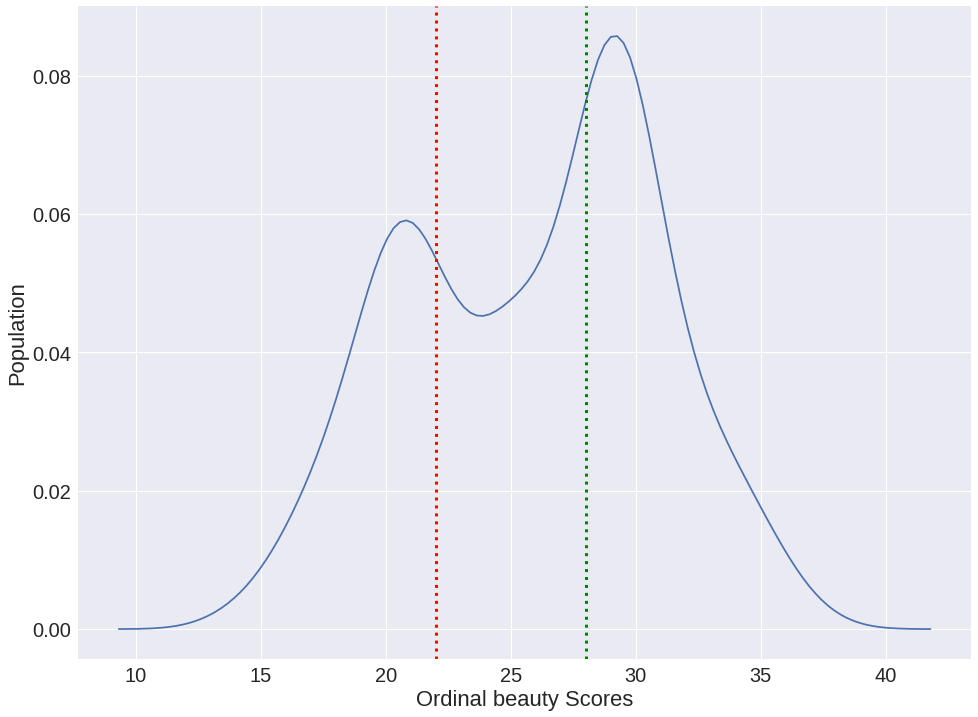
\includegraphics[width=0.7\columnwidth]{Plot/Trueskill.png}
	\caption{Frequency distribution of beauty scores. The red and green lines represent the thresholds below and above which images are considered ugly and beautiful. Conservatively, images in between are discarded.}
	\label{fig:Trueskill}
\end{figure}


\begin{figure*}[t!]
	\centering
	\hspace*{-5mm}
	\subfloat[]{
		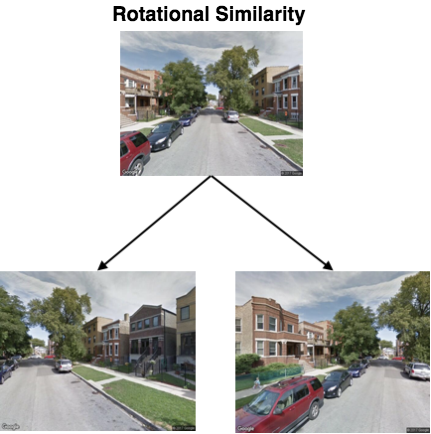
\includegraphics[width=0.5\textwidth, height = 8cm ]{Plot/rotationalSim.png}
		\label{fig:rotSim}
	}
	\subfloat[]{
		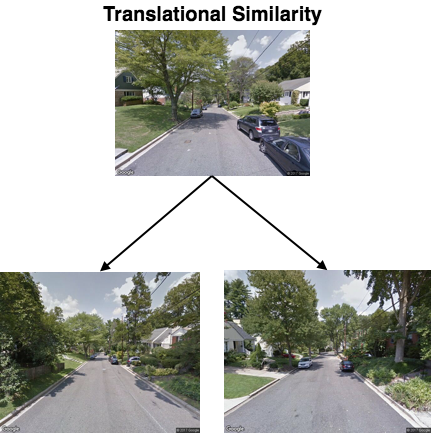
\includegraphics[width=0.5\linewidth, height = 8cm ]{Plot/transSim.png}
		\label{fig:transSim}
	}
	\vspace{-0.4cm}
	\caption{Two types of augmentation: (a) rotation of the Street Views camera (based on rotation); and (b) exploration of scenes at increasing distances (based on translation).}
	\vspace{-0.4cm}
\end{figure*}



\begin{figure}[t!]
	\centering
	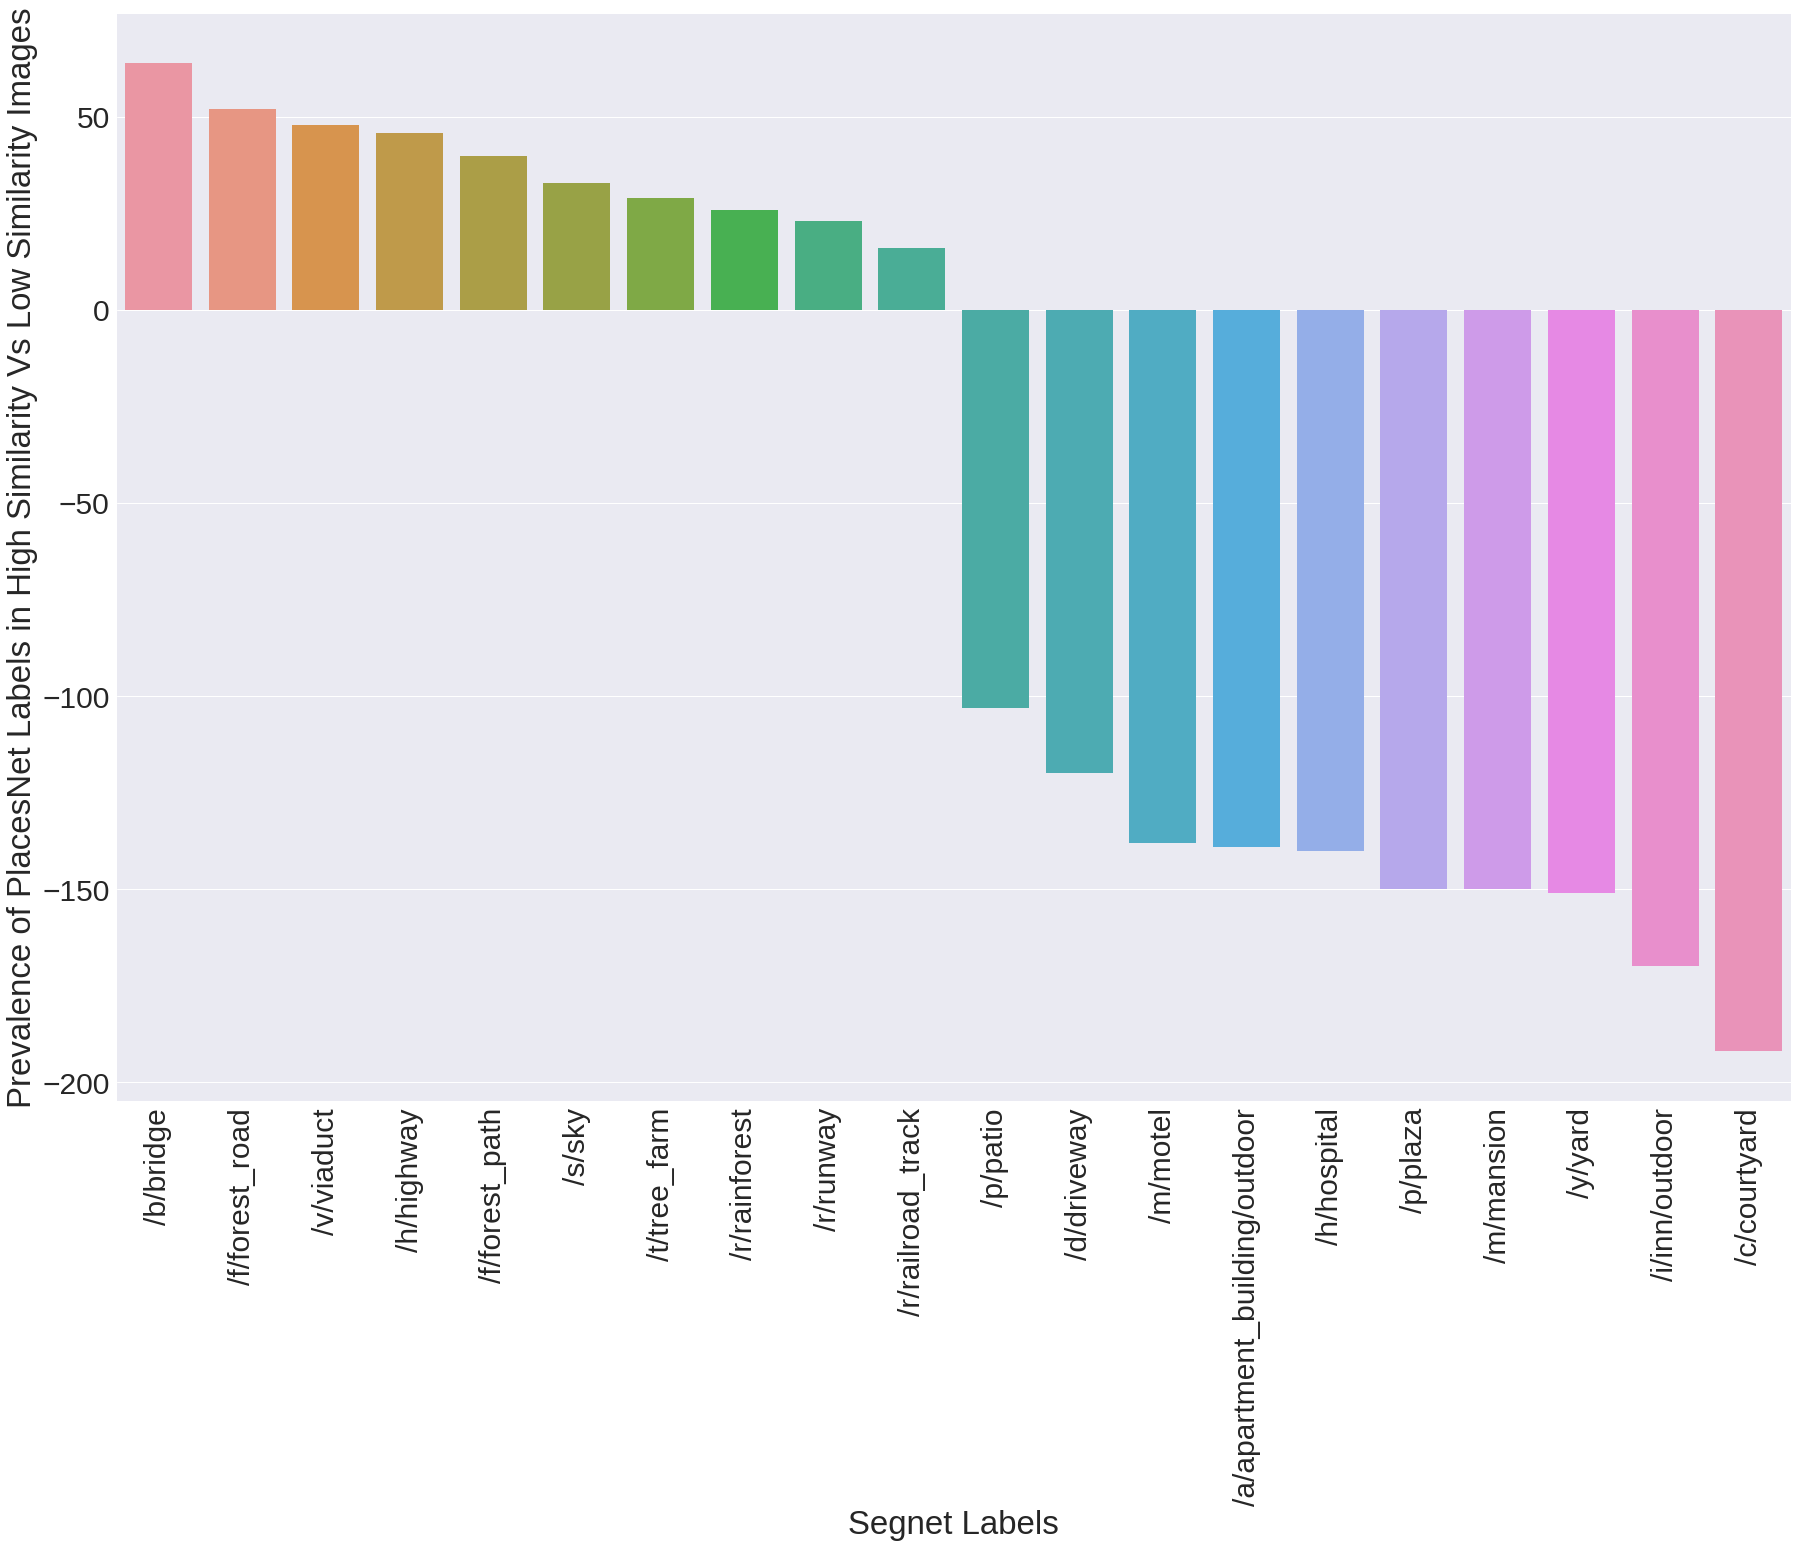
\includegraphics[width=\columnwidth]{Plot/SimilarityPlacesPrevalence.png}
	\caption{The types of scene that have greater propensity to be correctly augmented with similar scenes at increasing distances.}
	\label{fig:augmentationSimilarity}
\end{figure}




\begin{table}[t!]
	\centering
	\begin{tabular}{|c|c|}
		\hline
		\textbf{Augmentation} & \textbf{Accuracy (Percentage)}\\
		\hline
		None & 63 \\
		\hline
		Rotation  & 68 \\
		\hline
		Rotation + Translation  & 64 \\
		\hline
		Rotation + Conservative Translation & 73.5 \\
		\hline
	\end{tabular}
	\caption{Percentage accuracy for our beauty classifier trained on differently augmented sets of  urban scenes.}
	\label{tab:classifier}
    \vspace{-10mm}
\end{table}


%****************************************
\subsection*{Step 2 Training a beauty classifier}
\label{Sec:Classifier}
Having this highly curated set of labeled urban scenes, we are now ready to train classifier $C$ with labels reflecting our beauty assessments. We use the CaffeNet architecture, a modified version of AlexNet~\cite{krizhevsky2012imagenet,szegedy2015going}. \sj{The classifier network has a conventional convolutional network architecture, with 5 convolutional layers, interleaved with Max pooling and normalization layers. The network is terminated with two 4096 dimensional fully connected layers interleaved with dropout\cite{srivastava2014dropout} layers with dropout ration of 0.5, to prevent over-fitting of the network. Finally the classifier classifies the images into one of two classes (beautiful(1), ugly(0)) through a Softmax layer that computes probabilities of class membership.}

The training is done on a 70\% split of the data, and the testing on the remaining 30\%. All this is done on increasingly augmented sets of data. We start from our 20k images and progressively augment them with  the snapshots obtained with the 5-angle camera rotations, and then with the exploration of scenes at increasing distance $d \in \{10,20,40,60\}$ meters. The idea behind data augmentation is that accuracy would increase with it. Indeed it does (Table~\ref{tab:classifier}): it goes from 63\% on the set of original scenes to as much as 73.5\% on the set of fully augmented scenes, which is a notable increase in accuracy for such classes of classification tasks. As a baseline, we compare with the models trained by Dubey et.al in \cite{dubey2016deep} on the same seed data that we use for our pipeline. They report that their models perform at 70\% accuracy in the task of picking a beautiful image amongst any two given images. Albeit the set-up of our model is not to compare two images but just to classify a particular image in a binary class, this baseline shows that our model is showing a comparable performance in beauty classification. 
%As a baseline, we compared with the scenic-or-not model developed by Chanuki et.al \cite{seresinhe2017using}. Their model is different than ours because of the fact that their model generates scenic scores on a scale of 10, whereas ours is a binary classifier. Still for the sake of comparison, we measure the Kendall rank correlation, which is what they use for their measurements, between predicted and actual classes. Our model performs with a Kendall rank correlation of 0.43 which is comparable to their elastic net models. In so far, the facelift pipeline is agnostic of the classifier , which can be swapped out with a better performing one or with one trained for a different use case. 
%\ns{Can you cite a baseline comparison from state of the art? Less important but comment on why is accuracy the right metric? Why not precision for instance?}. 


%\begin{figure*}[h]
%	\centering
%	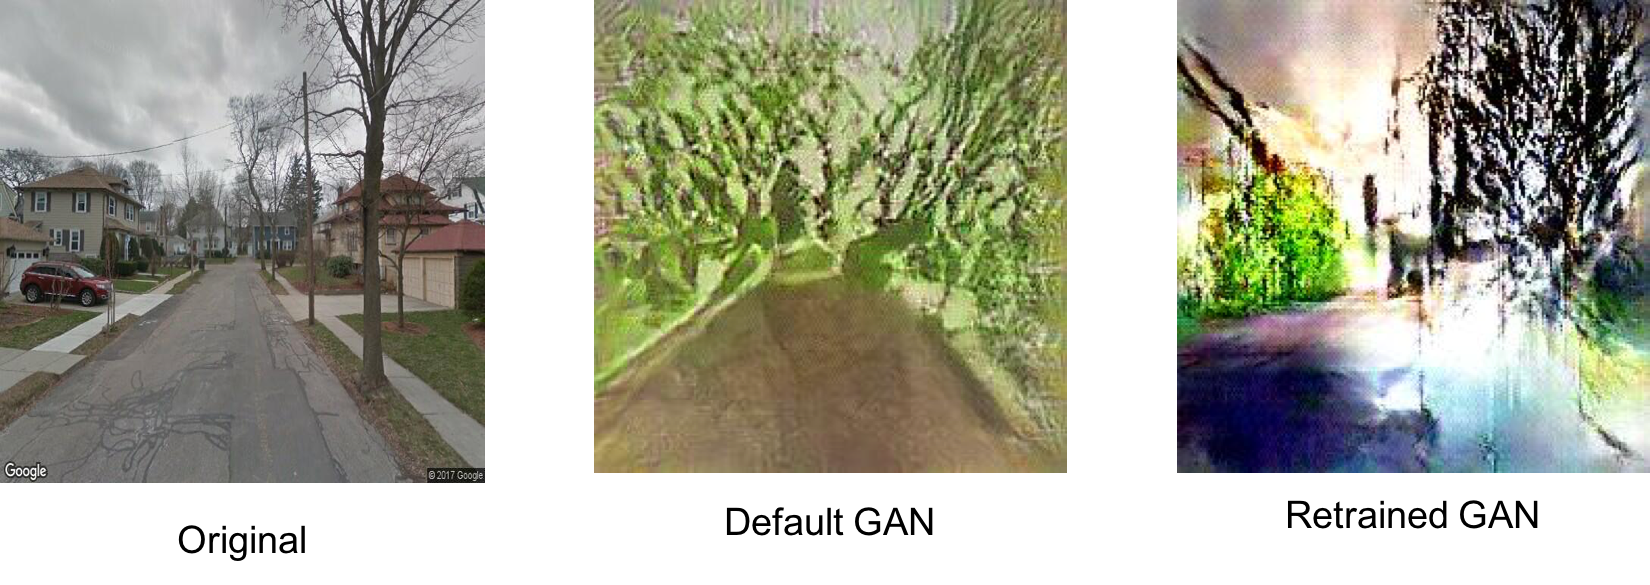
\includegraphics[width=0.5\linewidth]{Plot/GanCompare.png}
%	\caption{Comparison of using the Default ImageNet GAN against Custom trained GAN for Activation maximization. By re-training the GAN on the test dataset, we can see improvement in terms of structure and colours in the generated images}
%	\label{fig:GanComparison}
%\end{figure*}


%****************************************


\subsection*{Step 3 Generating a synthetic beautified scene}

\begin{figure}[t!]
    \centering
    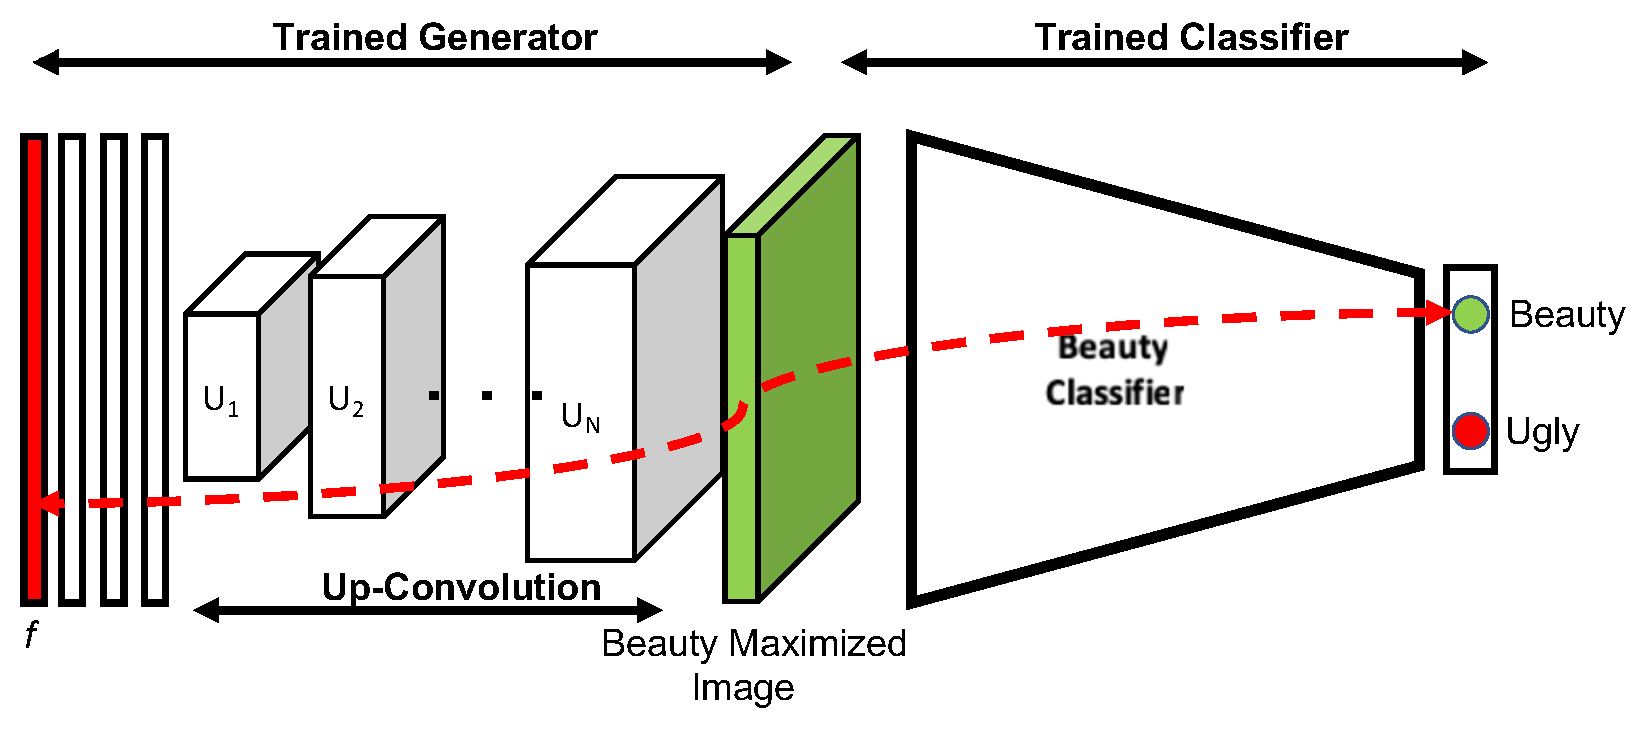
\includegraphics[width=\columnwidth]{Plot/AM_arch.pdf}
    \caption{\sj{The figure shows the architecture of the synthetic beauty generation pipeline. The pipeline is a Generator trained on all the curated streetview images in the dataset, cascaded with the trained classifier described in Section\ref{Sec:Classifier}. The green block represents the beauty maximized template $\hat{I_j}$. The red arrow describes the forward and backward pass that is optimized on.}}
    \label{fig:AM_arch}
\end{figure}

\begin{table}\sffamily
    \begin{tabular}{l*2{C}@{}}
        \toprule
        & Original & Generated \\ 
        \midrule
        & 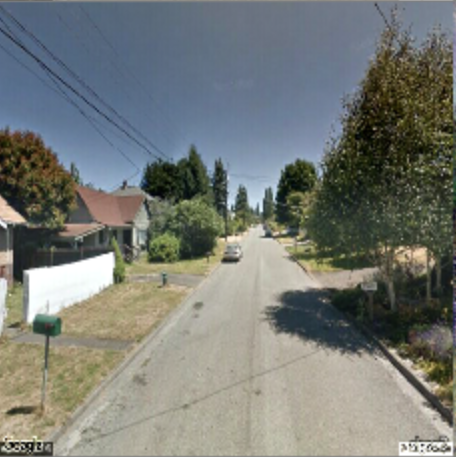
\includegraphics[width=11em]{Plot/GAN_examples/orig_1} & 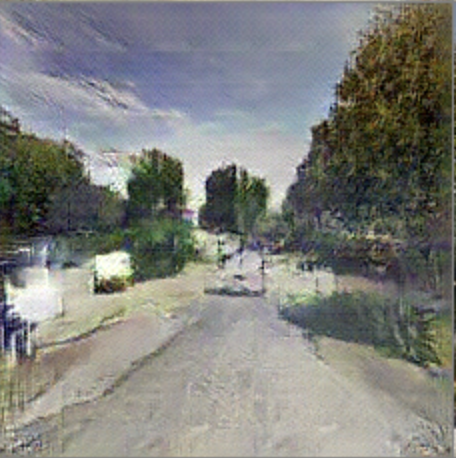
\includegraphics[width=11em]{Plot/GAN_examples/gan_1} \\ 
        & 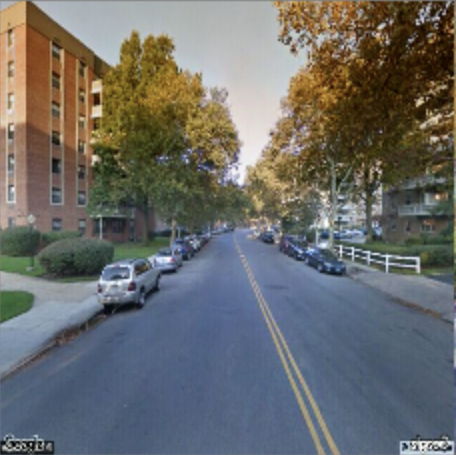
\includegraphics[width=11em]{Plot/GAN_examples/orig_2} & 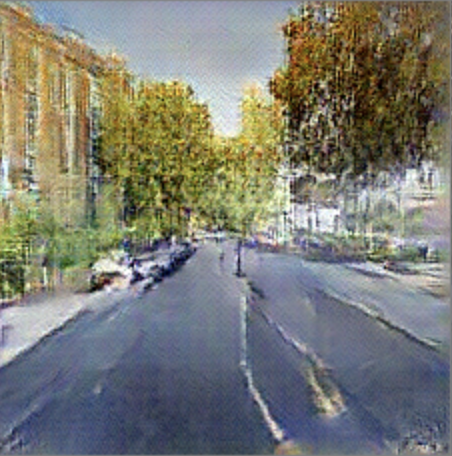
\includegraphics[width=11em]{Plot/GAN_examples/gan_2} \\ 
        & 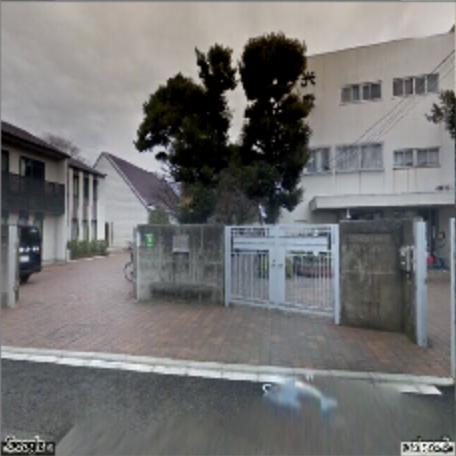
\includegraphics[width=11em]{Plot/GAN_examples/orig_3} & 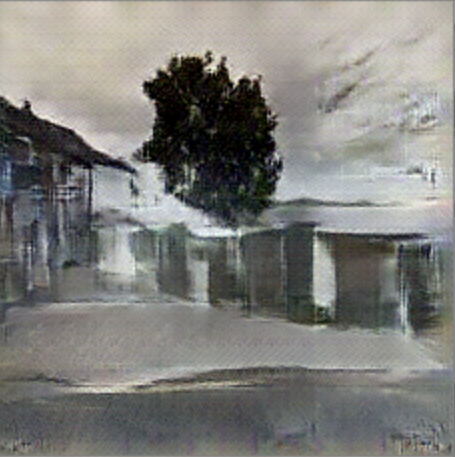
\includegraphics[width=11em]{Plot/GAN_examples/gan_3} \\ 
        
        \bottomrule 
    \end{tabular}
    \caption{ \sj{Sample examples of the outputs of the Generator network. The original scenes and the generated scenes are shown side by side. } }
    \label{fig:GanExample}
\end{table} 


Having this trained classifier at hand, we can then build a generator of synthetic beautified scenes. \sj{There are two components of this step. The first is to be able to generate synthetic scenes given an a-priori feature vector $f$, extracted from image $I_f$. For this component, we retrain the GAN described by Dosovitskiy and Brox\cite{dosovitskiy2016generating} on the curated urban scene dataset described in Section \ref{Sec:dataset}. This network is trained by optimizing along the principles of Generative Adverserial Networks\cite{goodfellow2014generative} i.e. maximizing the confusion for the discriminator between generated image $G(f)$ and real dataset images $I_f$. The resulting generator is able to reproduce synthetic urban scenes to a impressive detail. Figure \ref{fig:GanExample} shows a few examples of how the generator performs by comparing a real world image $I_f$, and the generated image $G(f)$. The second component is to cascade the trained generator with the trained classifier as described in Section\ref{Sec:Classifier} as shown in Figure \ref{fig:AM_arch}. This results in the end to end model } that, given the two classes ugly $y_i$ and beautiful $y_j$, transforms any original scene $I_i$ of class $y_i$ (e.g., ugly scene) into template scene $\hat{I_j}$ that maximizes class $y_j$ (e.g., beautified template scene). 

More specifically, given an input image $I_i$ known to be of class $y_i$  (e.g., ugly), our technique outputs  $\hat{I_j}$, which is a more beautiful version of it (e.g., $I_i$ is morphed  towards the average representation of a beautiful scene) while preserving $I_i$'s details. The technique does so using the ``Deep Generator Network for Activation Maximization'' (\emph{DGN-AM}) \cite{nguyen2016synthesizing}. Given an input image $I_i$, \emph{DGN-AM} iteratively re-calculates the color of $I_i$'s pixels in  a way  the output image $\hat{I_j}$  both maximizes  the  activation of neuron $y_j$ (e.g., the ``beauty neuron'') and looks ``photo realistic'',  which is done by conditioning the maximization to an ``image prior''. This is equivalent to finding the feature vector $f$ that maximizes the following expression:
\begin{equation}
\hat{I_j} =G( f ) : \underset{f}{\arg\max}(C_{j}(G(f))-\lambda||f||)
\end{equation}
where:
\begin{itemize}
\item $G(f)$ is the image synthetically generated from the candidate feature vector $f$;
\item $C_j(G(f))$ is the activation value of neuron $y_j$ in the scene classifier $C$ (the value to be maximized);
\item $\lambda$ is a $L_2$ regularization term.
\end{itemize}
Here the initialization of $f$ is key. If $f$ were to be initialized with random noise, then the resulting $G(f)$ would be the average representation of category $y_j$ (of, e.g., beauty). Instead, since $f$ is initialized with $I_i$, then the resulting $G(f)$ is $I_i$'s version ``morphed to become more beautiful''.
\sj{The legibility of the transformed image is highly dependent on the initial state of the neural activation that you are trying to maximize. Maximizing beauty of an already beautiful image, would yield in a saturated, illegible template $\hat{I_j}$. For this reason, to generate an image, that maximizes the beauty neuron in the classifier $C$ , you need to supply an apriori image that most definitely lies in the class $y_i$. The constraint is reverse for maximizing for class $y_i$} 
%Figure \ref{fig:BeautyExample} shows the activation maximization output in the center.

%****************************************
\subsection*{Step 4 Returning a realistic beautified scene}
 We now have template scene $\hat{I_j}$ (which is a synthetic beautified version of original scene $I_i$) and need to retrieve a realistic looking version of it. We do so by: \emph{i)} representing each of our original scenes in Step 1 (including $\hat{I_j}$) as a 4096 dimensional feature vector derived from the FC7 layer of the PlacesNet \cite{zhou2014learning}; \emph{ii)} computing the distance (as $L_2$ Norm) between $\hat{I_j}$'s feature vector and each of the original scene's feature vector; and \emph{iii)} selecting the original scene most similar (smaller distance) to $\hat{I_j}$. This results into the selection of the beautified scene $I_j$.
 
 
 %****************************************
\subsection*{Step 5 Identifying  characterizing urban elements}
Since original scene $I_i$ and beautified scene $I_j$ are real scenes and we make sure that they maintain the same structural characteristics (e.g., point of view, layout), we can easily compare them in terms of presence or absence of SegNet's and PlacesNet's labels. That is, we can determine how the original scene and its beautified version differ in terms of urban design elements. This step required us to develop metrics inspired from urban design literature, to quantify the changes in elements. A detailed description of the characterization and evaluation would follow in Section \ref{sec:evaluation}
 
 
%\begin{figure*}[h]
%	\centering
%	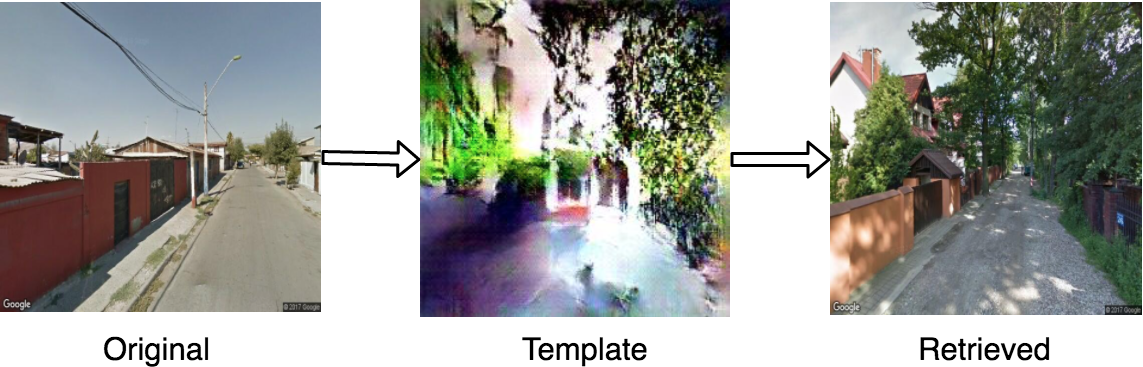
\includegraphics[width=\linewidth]{Plot/Example.png}
%	\caption{Example of ``FaceLifting''.}
%	\label{fig:BeautyExample}
%\end{figure*}


	\begin{table}\sffamily
	\begin{tabular}{l*3{C}@{}}
		\toprule
		 & Original ($I_i$) & Latent Beauty representation ($\hat{I_j}$) & Beautified ($I_j$) \\ 
		\midrule
		& 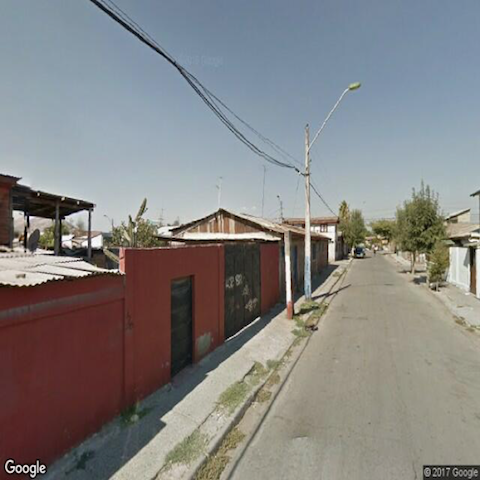
\includegraphics[width=11em]{Plot/examples/u_9} & 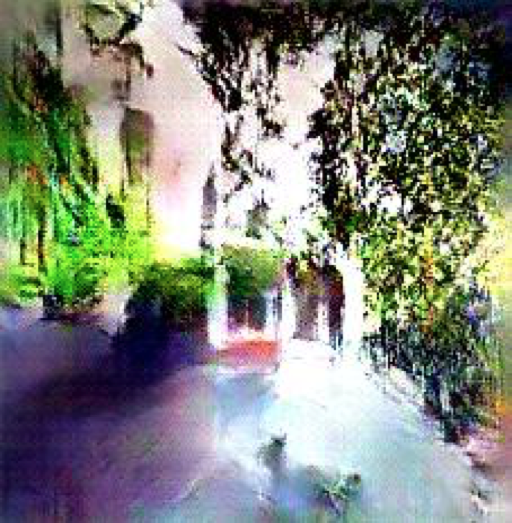
\includegraphics[width=11em]{Plot/examples/t_9} &  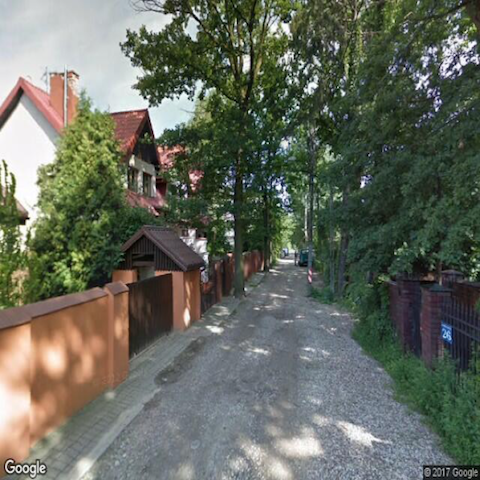
\includegraphics[width=11em]{Plot/examples/b_9} \\ 
%		& 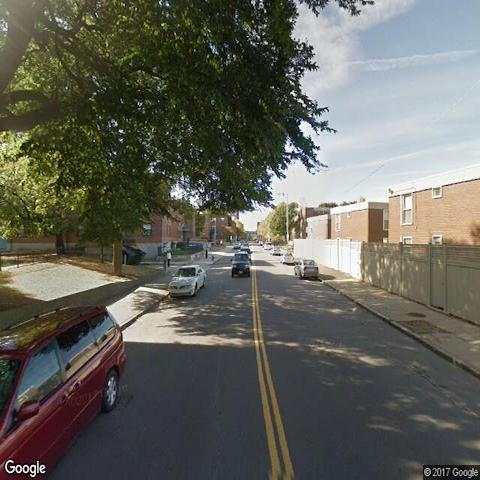
\includegraphics[width=11em]{Plot/examples/u_1} & 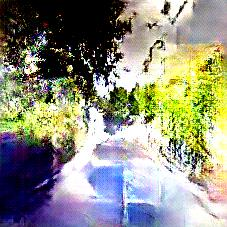
\includegraphics[width=11em]{Plot/examples/t_1} &  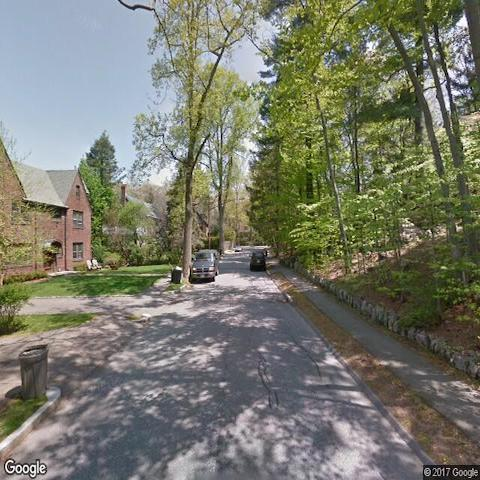
\includegraphics[width=11em]{Plot/examples/b_1} \\ 
%		& 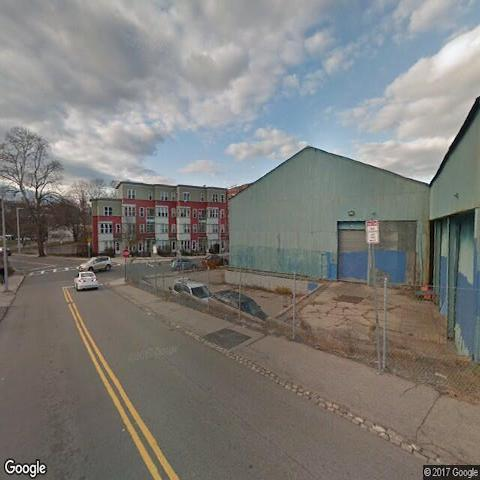
\includegraphics[width=11em]{Plot/examples/u_2} & 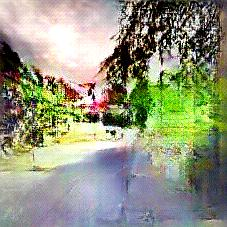
\includegraphics[width=11em]{Plot/examples/t_2} &  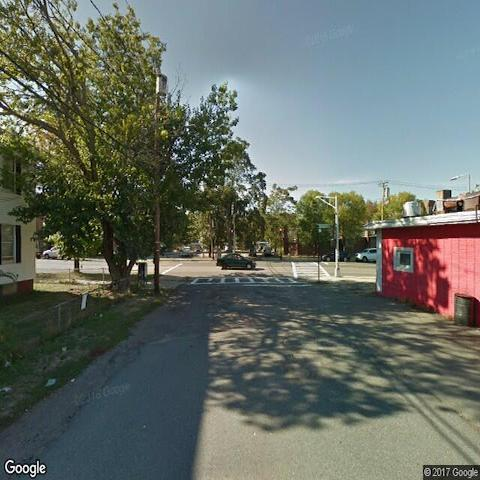
\includegraphics[width=11em]{Plot/examples/b_2} \\ 
%		& 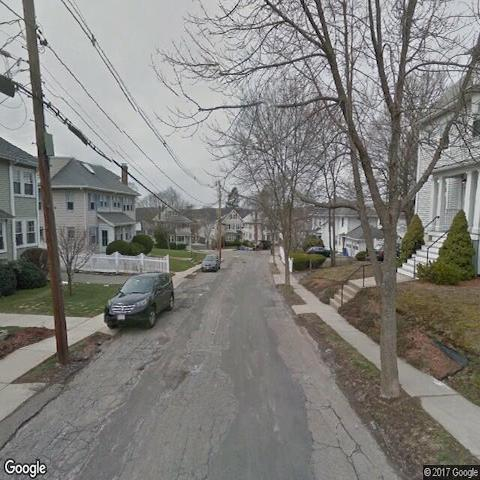
\includegraphics[width=11em]{Plot/examples/u_3} & 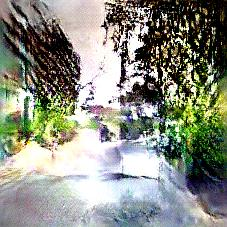
\includegraphics[width=11em]{Plot/examples/t_3} &  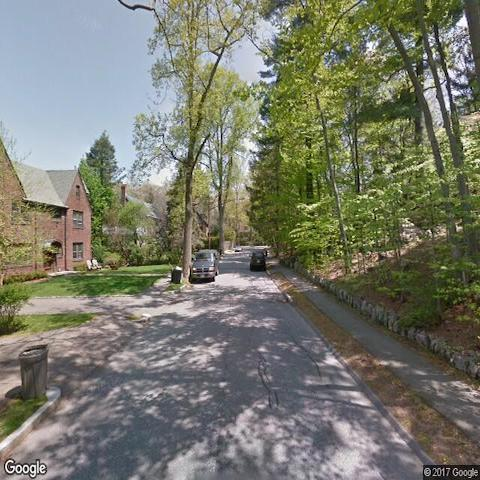
\includegraphics[width=11em]{Plot/examples/b_3} \\ 
		& 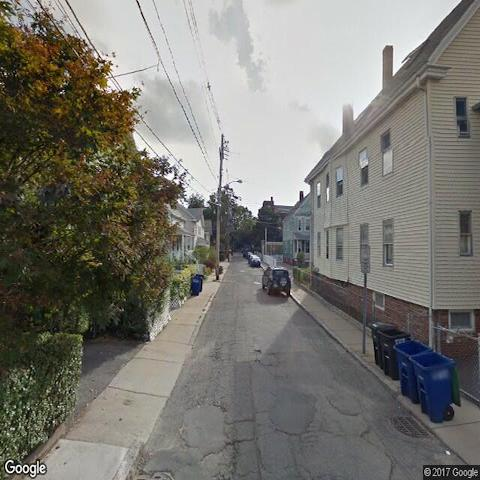
\includegraphics[width=11em]{Plot/examples/u_4} & 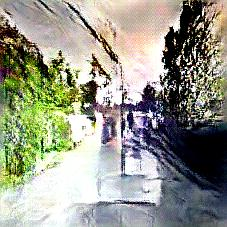
\includegraphics[width=11em]{Plot/examples/t_4} &  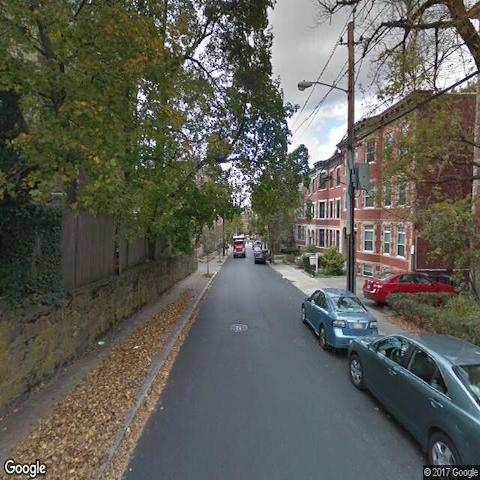
\includegraphics[width=11em]{Plot/examples/b_4} \\ 
		& 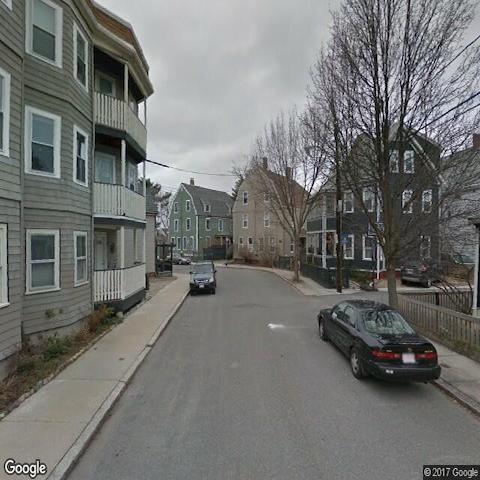
\includegraphics[width=11em]{Plot/examples/u_5} & 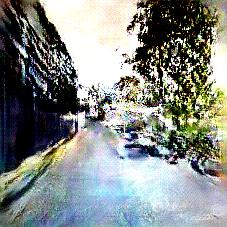
\includegraphics[width=11em]{Plot/examples/t_5} &  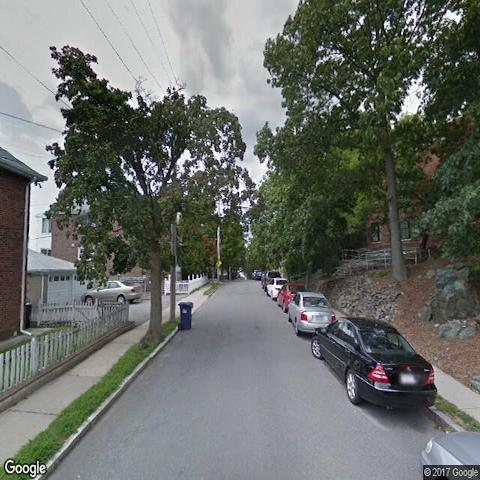
\includegraphics[width=11em]{Plot/examples/b_5} \\ 
%		& 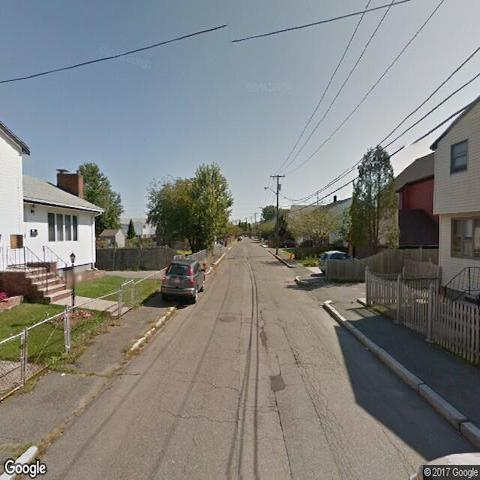
\includegraphics[width=11em]{Plot/examples/u_6} & 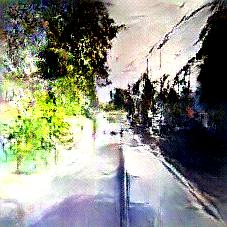
\includegraphics[width=11em]{Plot/examples/t_6} &  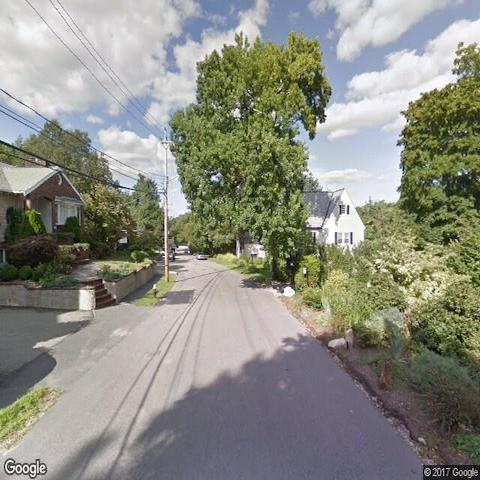
\includegraphics[width=11em]{Plot/examples/b_6} \\ 
		& 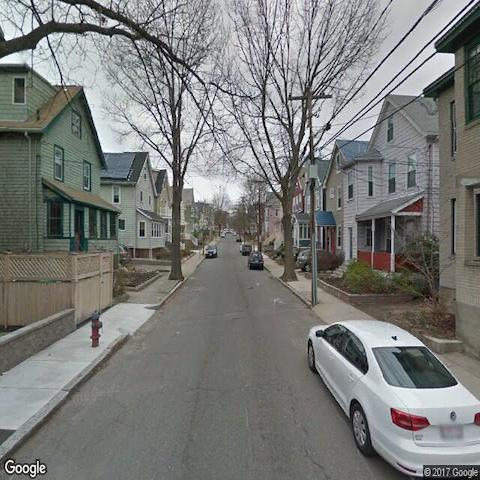
\includegraphics[width=11em]{Plot/examples/u_7} & 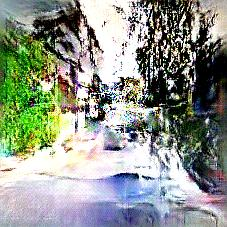
\includegraphics[width=11em]{Plot/examples/t_7} &  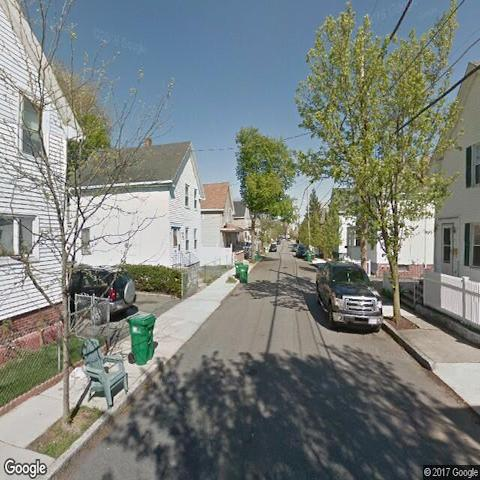
\includegraphics[width=11em]{Plot/examples/b_7} \\ 
		& 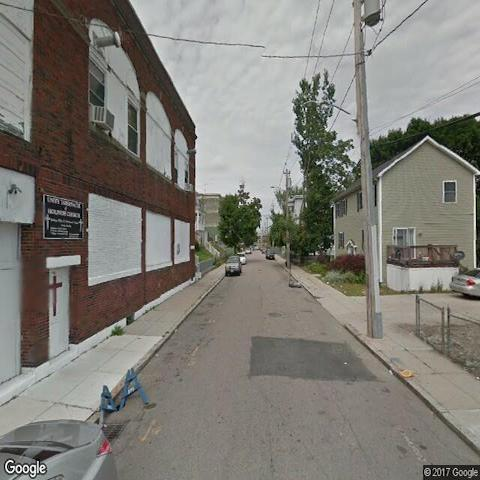
\includegraphics[width=11em]{Plot/examples/u_8} & 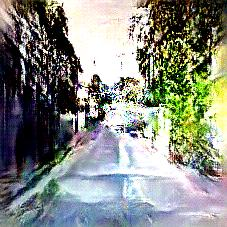
\includegraphics[width=11em]{Plot/examples/t_8} &  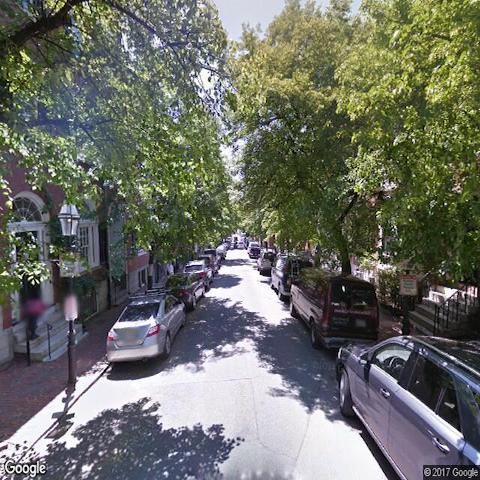
\includegraphics[width=11em]{Plot/examples/b_8} \\ 
		\bottomrule 
	\end{tabular}
	\caption{ The table showcases examples of the``FaceLifting'' process. It is worth observing that the process of beautification prefers greenery, narrow roads and  pavements }
	\label{fig:BeautyExample}
\end{table} 


\section{Evaluation}
\label{sec:evaluation}

The goal of FaceLift is to transform existing urban scenes into versions that: \emph{i)} people perceive more beautiful; \emph{ii)} contain urban elements typical of great urban spaces; \emph{iii)} are easy to interpret; and \emph{iv)} architects and urban planners find useful. To ascertain whether FaceLift meets that composite goal, we answer the following questions next: 

\begin{description}
\item{\textbf{Q1}} Do individuals perceive``FaceLifted'' scenes to be beautiful?

\item{\textbf{Q2}}  Does our framework produce scenes that possess urban elements typical of great spaces?

\item{\textbf{Q3}}  Which urban elements are mostly associated with beautiful scenes?

\item{\textbf{Q4}}  Do architects and urban planners find FaceLift useful?

\end{description}


\subsection*{Q1 People's perceptions of beautified scenes}
To ascertain whether FaceLifted scenes are perceived by individuals as they are supposed to, we run a crowd-sourcing experiment on Amazon Mechanical Turk.  We randomly select 200 scenes, 100 beautiful and 100 ugly  (taken at the bottom 10 and top 10 percentiles of the Trueskill's score distribution of Figure~\ref{fig:Trueskill}). Our framework then transforms each ugly scene into its beautified version, and each beautiful scene into its corresponding `uglified'. These scenes are arranged into pairs, each of which contains the original scene and its beautified or uglified version. On  Mechanical Turk, we only select verified masters for our crowd-sourcing workers (those with an approval rate above 90\% during the past 30 days), pay them \$0.1 per  task,  and ask each of them to choose the beautiful scene for given pairs.  We make sure to have at least 3 votes for each scene pair. Overall, our workers end up selecting the scenes that are actually beautiful 77.5\% of the times, suggesting that FaceLifted scenes are correctly perceived most of the times.


\subsection*{Q2 Are beautified scenes great urban spaces?}
To answer that question, we need to understand what makes a space great. After a careful review of the urban planning literature, we identify four factors~\cite{ewing2013measuring,alexander1977pattern} (summarized in Table~\ref{tab:Design_metrics}): great places mainly tend to be walkable, offer greenery, feel cozy, and be visually rich. 


\begin{table*}[h]
	\centering
	
	\resizebox{\linewidth}{!}{%
		\begin{tabular}{|c|p{10cm}|}
			\hline
			\textbf{Metric} & \textbf{Description}\\
			\hline
			Walkability  & Walkable streets increase the social capital of a place,  and they appeal to the exploring nature of the human psyche~\cite{ewing2013measuring,quercia15thedigital,speck12}.\\
			\hline
			Green Spaces & The presence of greenery has repeatedly been found to impact people's well being \cite{alexander1977pattern}. Under certain conditions, it could also promote social interactions~\cite{quercia2014aesthetic}. This suggest that not all greenery has to be considered in the same way though: dense forests or unkempt greens might well have a negative impact~\cite{jacobs1961death}. \\
			\hline		
			\sj{Landmarks} & \sj{Loosing a bearing in the city is not a very pleasant experience. Hence presence of recognisable and  guiding landmarks influences the perception of an urban space \cite{lynch1960image,quercia2014aesthetic,ewing2013measuring}.}\\
			\hline
			Privacy-Openness &  A sense of privacy (as opposed to a sense of openness) impacts a place's perception~\cite{ewing2013measuring}.\\ 
			\hline
			Visual Complexity & Visual complexity is a measure of how diverse a urban scene is in terms of design materials, textures, and objects~\cite{ewing2013measuring}. \sj{We perceive complexity in an `inverted-U' fashion, which means we prefer medium complexity over too little or too much for finding a place pleasant\cite{ulrich1983aesthetic}} \\
			\hline
	\end{tabular}}
	\caption{Urban Design Metrics}
	\label{tab:Design_metrics}
	%        \vspace{-5mm}
\end{table*}


To automatically extract visual cues related to these four factors, we select 500 ugly scenes and 500 beautiful ones at random, transform them into their opposite aesthetic qualities (i.e., ugly ones are beautified, and beautiful ones are `uglified'), and compare which urban elements related to the four factors distinguish uglified scenes from beautified ones. 

We extract labels from each of our 1,000 scenes using two image classifiers. First, using PlacesNet~\cite{zhou2014learning}, we label each of our scenes according to a classification containing 205 labels (reflecting, for example, landmarks, natural elements), and retain the five labels with highest confidence scores for the scene. Second, using Segnet~\cite{badrinarayanan2015segnet}, we  label each of our scenes according to a classification containing 12 labels. Segnet is trained on dash-cam images, and classifies each scene pixel with one of these twelve labels: road, sky, trees,  buildings, poles, signage, pedestrians, vehicles, bicycles, pavement, fences, and road markings. 

\begin{figure}[h]
	\centering
	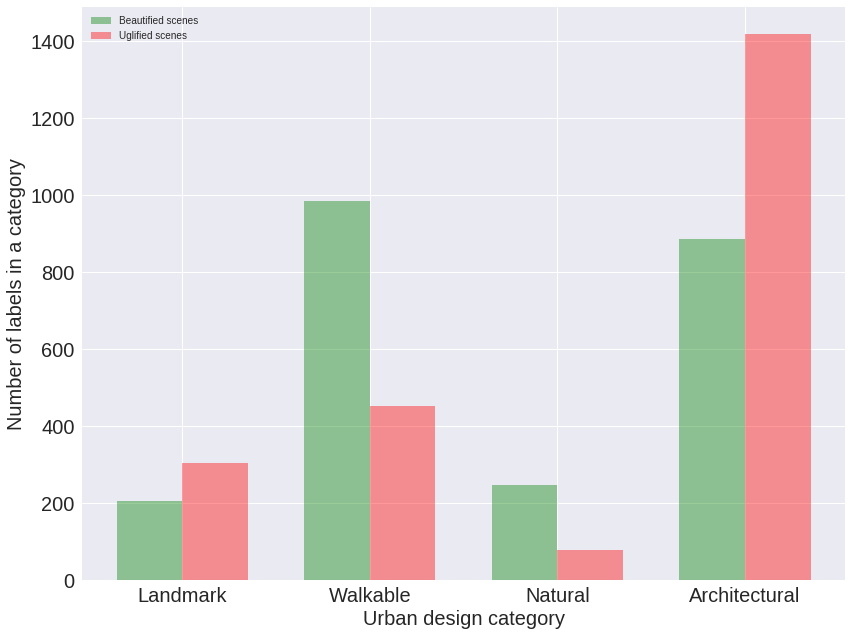
\includegraphics[width=\columnwidth]{Plot/taxonomyCount.png}
	\caption{Number of labels in specific urban design categories (on the $x$-axis) found in beautified scenes as opposed to those found in uglified scenes.}
	\label{fig:taxonomyCount}
\end{figure}


\begin{figure}[h]
	\centering
	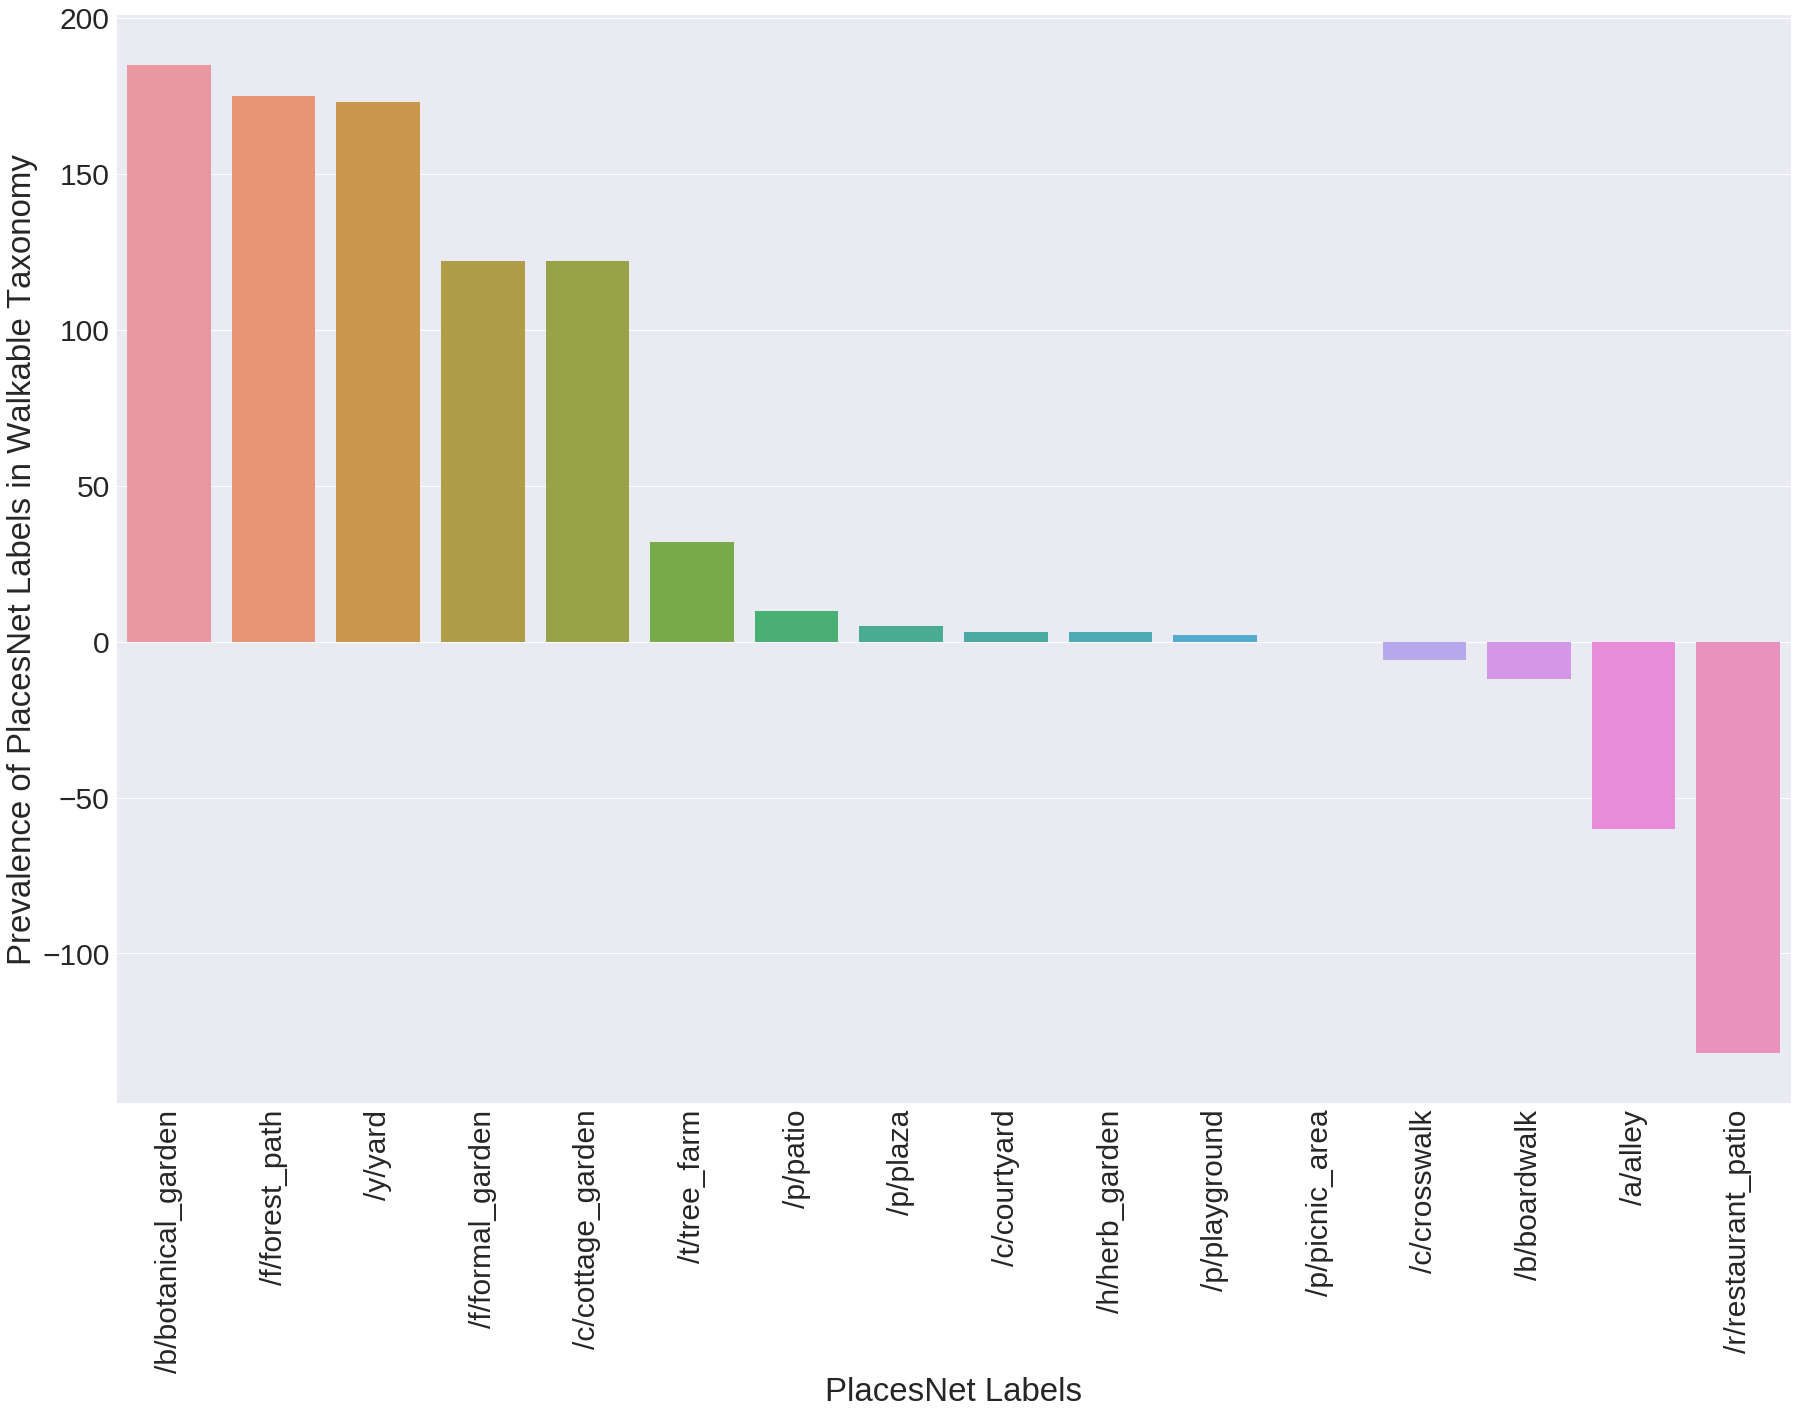
\includegraphics[width=\columnwidth]{Plot/walkable_taxonomy.png}
	\caption{Count of specific walkability-related labels  (on the $x$-axis) found in beautified scenes minus the count of the same labels found in uglified scenes.}
	\label{fig:WalkableTnomy}
\end{figure}


Having these two ways of labeling scenes, we can now test whether the expectations set by the literature describing metrics of great urban spaces (Table~\ref{tab:Design_metrics}) are  met in the FaceLifted scenes. 


%**************************************************
\mbox{ } \\
\noindent
\emph{H1 Beautified scenes tend to be walkable.}
We manually select only the PlacesNet labels that are related to walkability. These labels include, for example, \textit{abbey, plaza, courtyard, garden, picnic area, \textrm{and} park}. To test hypothesis \emph{H1}, we count the number of walkability-related labels found in beautified scenes as opposed to those found in uglified scenes (Figure~\ref{fig:taxonomyCount}): the former contain twice as many walkability labels than the latter. We then determine which types of scenes are associated with beauty (Figure~\ref{fig:WalkableTnomy}). Unsurprisingly, beautified scenes tend to show gardens, yards, and small paths. By contrast, uglified ones tend to show built environment features such as shop fronts and broad roads. 


\mbox{ } \\
%**************************************************
\noindent
\emph{H2 Beautified scenes tend to offer green spaces.}
We manually select only the PlacesNet labels that are related to greenery. These labels include, for example, \textit{fields, pasture, forest, ocean, and beach}. Then, in our 1,000 scenes, to test hypothesis \emph{H2}, we count the number of nature-related labels found in beautified scenes as opposed to those found in uglified scenes (Figure~\ref{fig:taxonomyCount}): the former contain more than twice as many nature-related labels than the latter.  To test this hypothesis further, we compute the fraction of `tree' pixels (using SegNet's label `tree') in beautified and uglified scenes, and  find that beautification adds  32\% of tree pixels, while uglification removes 17\% of them. 


\begin{figure*}[!t]
	\centering
	\hspace*{-5mm}
	\subfloat[]{
		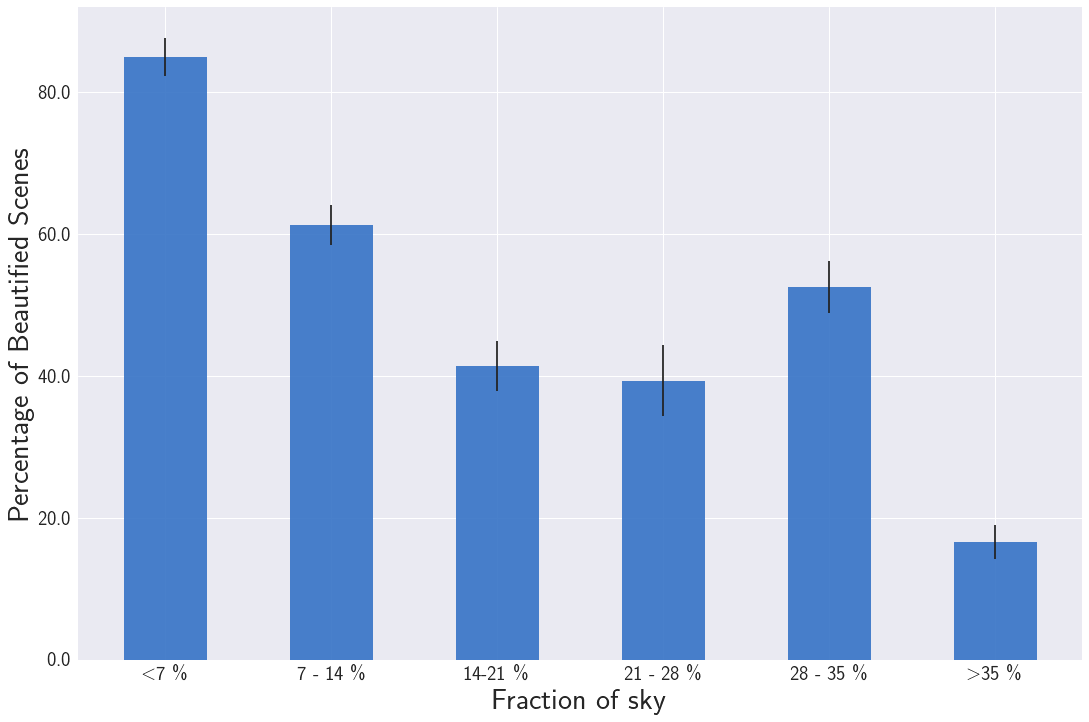
\includegraphics[width=0.45\textwidth, height = 5cm ]{Plot/BinnedPlot.png}
		\label{fig:skyBinned}
	}
	\subfloat[]{
		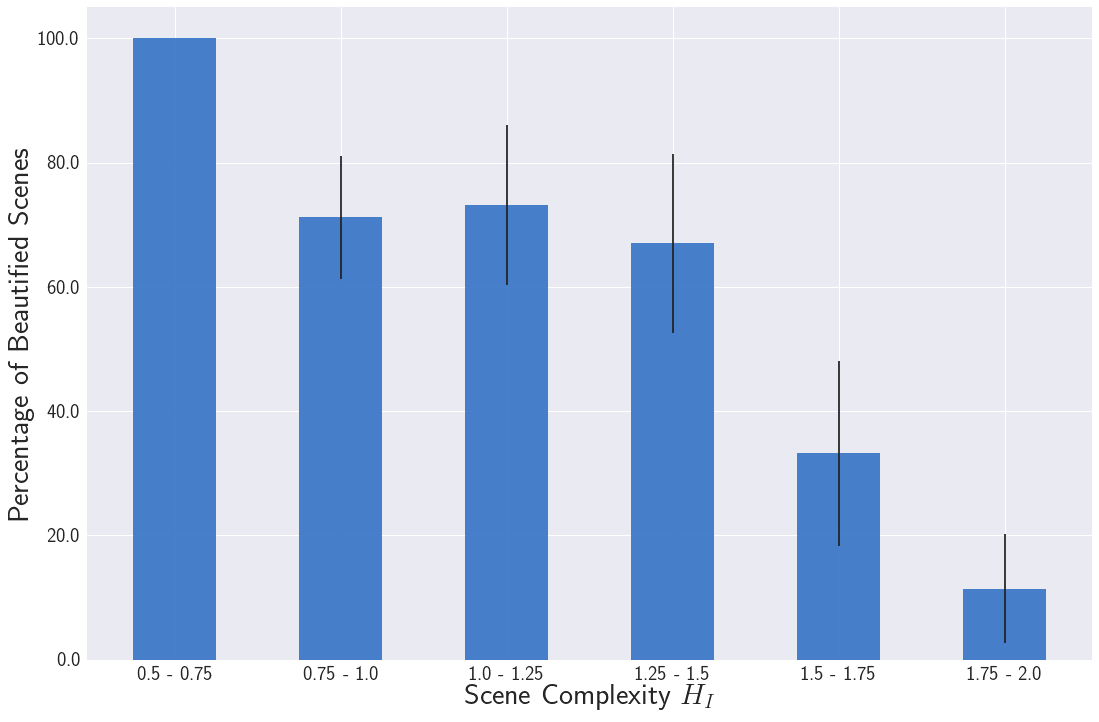
\includegraphics[width=0.45\linewidth, height = 5cm ]{Plot/binnedPlot_complexity.png}
		\label{fig:complexity}
	}
\vspace{-0.4cm}
\label{fig:bin_figures}
\caption{The percentage of scenes ($y$-axis): (a) having an increasing presence of sky (on the $x$-axis); and (b) having an increasing level of visual richness  (on the $x$-axis). The error bars represent standard errors obtained by random re-sampling of the data for 500 iterations. }
\vspace{-0.4cm}
\end{figure*}



\mbox{ } \\
%**************************************************
\noindent
\emph{H3 Beautified scenes tend to feel private and `cozy'.}
To  test hypothesis \emph{H3}, we count the fraction of pixels that Segnet labeled  as `sky' and show the results in a bin plot in Figure~\ref{fig:skyBinned}:  the $x$-axis has six bins (each of which represents a given range of sky fraction), and the $y$-axis shows the percentage of beautified \emph{vs.} uglified scenes that fall into each bin.  Beautified scenes tend to be cozier (lower sky presence) than the corresponding original scenes.


\mbox{ } \\
%**************************************************
\noindent
\emph{H4 Beautified scenes tend to be visually rich}
To quantify to which extent scenes are visually rich, we measure their visual complexity~\cite{ewing2013measuring} as  the amount of disorder in terms of distribution of (Segnet) urban elements in the scene: 
\begin{equation}
H(X) = -\sum p(i)\log p(i)
\label{eq:entropy} 
\end{equation}
where $i$ is the $i^{th}$ Segnet's label. The total number of labels is twelve. The higher $H(X)$, the  higher the scene's entropy, that is, the higher the scene's complexity. \sj{It has been proposed, that the perception of aesthetics or pleasantness follows an `inverted U' shape\cite{ulrich1983aesthetic}.} To test hypothesis \emph{H4}, we show the percentage of scenes that fall into a complexity bin  (Figure~\ref{fig:complexity}): beautified scenes are of low to medium complexity, while uglified ones are of high complexity.



%**************************************************
\subsection*{Q3 Urban elements of beautified scenes}

\begin{table}[t!]
	\centering
	\resizebox{\linewidth}{!}{%
	\begin{tabular}{|c|c|c|c|c|}
		\hline
		\textbf{Pair of urban elements} & \textbf{$\beta_1$}  & \textbf{$\beta_2$} & \textbf{$\beta_3$}  & Error Rate (Percentage)\\
		\hline
        \hline
		Buildings - Trees & -0.032 & 0.084  & 0.005  & 12.7 \\
		\hline
		Sky - Buildings & -0.08 & -0.11 & 0.064 & 14.4 \\
		\hline
		Roads - Vehicles  & -0.015  & -0.05 & 0.023  & 40.6 \\
		\hline
		Sky - Trees & 0.03 & 0.11 & -0.012 & 12.8  \\
		\hline
		Roads - Trees & 0.04  & 0.10 &  -0.031  & 13.5  \\
		\hline
		Roads - Buildings & -0.05  & -0.097  &  0.04  & 20.2  \\
		\hline
	\end{tabular}
	}
	\caption{Coefficients of logistic regressions run on one pair of predictors at the time.}
	\label{tab:regressioncoef}
    \vspace{-10mm}
\end{table}


To determine which urban elements are the best predictors of urban beauty and the extent to which they are so, we run a logistic regression, and, to ease interpretation, we do so on one pair of predictors at the time: 
\begin{equation}
Pr(\textrm{beautiful}) = logit^{-1}(\alpha + \beta_1 * V_1 + \beta_2 * V_2  + \beta_3 * V_{1}.V_{2} )
\label{eq:regression} 
\end{equation}
where $V1$ is the fraction of the scene's pixels marked with one Segnet's label, say, ``buildings'' (over the total number of pixels),  and $V2$ is the fraction of the scene's pixels marked with another label, say, ``trees''. The result consists of three beta coefficients: $\beta_1$ reflects $V1$'s contribution in predicting beauty,  $\beta_2$ reflects $V2$'s contribution, and $\beta_3$ is the interaction effect, that is, it reflects the contribution of the dependency of $V1$ and $V2$ in predicting beauty. We run logistic regressions on the five factors that have been found to be most predictive of urban beauty~\cite{quercia2014aesthetic, ewing2013measuring, alexander1977pattern}, and show the results in Table~\ref{tab:regressioncoef}.


Since we are using logistic regressions, the quantitative interpretation of the beta coefficients is eased by the ``divide by 4 rule''~\cite{vaughn2008data}: we can take $\beta$ coefficients and ``divide them by 4 to get an upper bound of the predictive difference corresponding to a unit difference'' in beauty~\cite{vaughn2008data}. For example, take the results in the first row of Table~\ref{tab:regressioncoef}. In the model $Pr(beautiful) = logit^{-1}(\alpha - 0.032 \cdot buildings + 0.084 \cdot trees + 0.005 \cdot  buildings \cdot trees)$, we can divide - 0.032/4 to get -0.008: a difference of 1 in the fraction of pixels being buildings corresponds to no more than a 0.8\% \emph{negative} difference in the probability of the scene being beautiful. In a similar way, a difference of 1 in the fraction of pixels being trees corresponds to no more than a 0.021\% \emph{positive} difference in the probability of the scene being beautiful. By considering the remaining results in Table~\ref{tab:regressioncoef}, we find that, across all pairwise comparisons, trees is the most positive element associated with beauty, while roads and buildings are the most negative ones. Since these results go in the direction one would expect, one might conclude that the scenes beautified by our framework are in line with previous literature, adding further external validity to our work. 




%**************************************************
\subsection*{Q4 Do architects and urban planners find it useful?}

\begin{table}[t!]
	\centering
	\resizebox{\linewidth}{!}{%
		\begin{tabular}{|c|c|c|c|c|c|}
			\hline
			\textbf{Use case} & \textbf{Definitely Not}  & \textbf{Probably Not} & \textbf{Probably}  & \textbf{Very Probably} & \textbf{Definitely}\\
			\hline
			\hline
			Decision Making & 4.8\% & 9.5\%  & 38\%  &  28.6\% & 19\%\\
			\hline
			Participatory Urban Planning & 0\% & 4.8\%  & 52.4\%  &  23.8\% & 19\%\\
			\hline
			Promote Green Cities & 4.8\% & 0\%  & 47.6\%  &  19\% & 28.6\%\\
			\hline
		\end{tabular}
	}
	\caption{Urban experts polled about the extent to which an interactive map of ``FaceLifted'' scenes promotes: (a) decision making; (b) citizen participation in urban planning; and (c) promotion of green cities}
	\label{tab:useCases}
	\vspace{-10mm}
\end{table}


%\begin{figure*}[!t]
%	\centering
%	\hspace*{-5mm}
%	\subfloat[]{
%		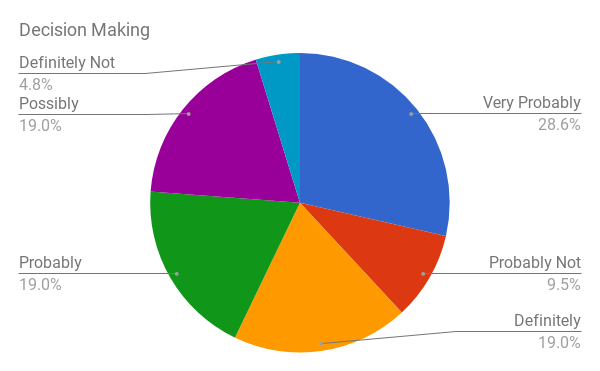
\includegraphics[width=0.3\textwidth ]{Plot/DecisionMaking.png}
%		\label{fig:decision}
%	}
%	\subfloat[]{
%		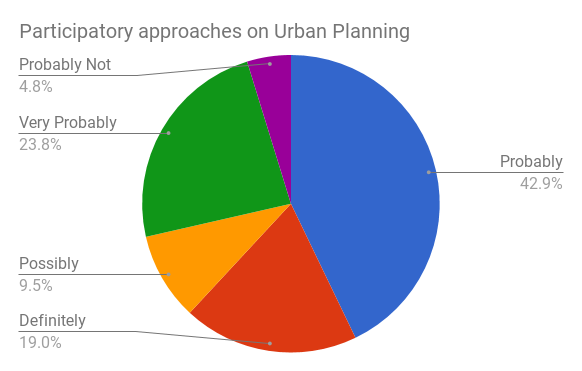
\includegraphics[width=0.3\linewidth ]{Plot/ParticipationUrbanPlanning.png}
%		\label{fig:participation}
%	}
%	\subfloat[]{
%		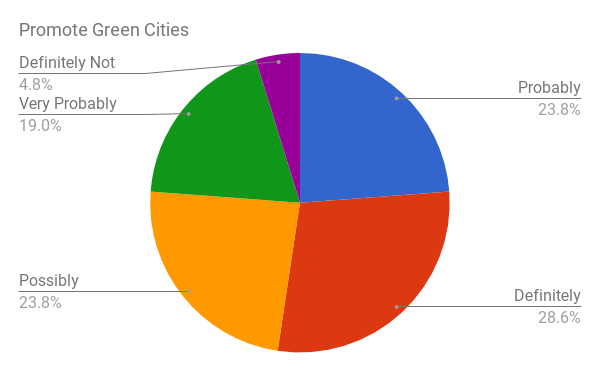
\includegraphics[width=0.3\linewidth ]{Plot/PromoteGreenCities.png}
%		\label{fig:promotion}
%	}
%%	\vspace{-0.4cm}
%	\caption{Urban experts polled about the extent to which an interactive map of ``FaceLifted'' scenes promotes: (a) decision making; (b) citizen participation in urban planning; and (c) promotion of green cities.\ns{Pie charts are not advisible. The labels are too small. You can perhaps replace this with a table.}}
%	\label{fig:pies}
%	\vspace{-0.4cm}
%\end{figure*}


\begin{figure}[t!]
	\centering
	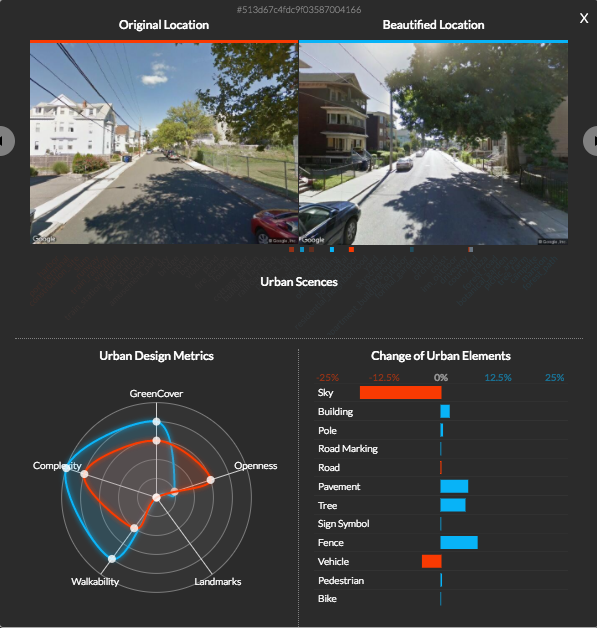
\includegraphics[width=\columnwidth]{Plot/UI.png}
	\caption{Interactive map of FaceLifted scenes in Boston.}
	\label{facelift-UI}
\end{figure}



To ascertain whether practitioners find FaceLift potentially useful, we built an interactive map of the city of Boston in which, for  selected points, we showed pairs of urban scenes before/after beautification (Figure~\ref{facelift-UI}). We then sent that map along with a survey to 20 experts in architecture, urban planning, and data visualization around the world. \sj{Being experts in their respective fields, we wanted the survey takers to express a clear opinion about the utility of such a technology in their areas of practice. In accordance with this constraint, we designed the survey based on a non neutral response Likert scale, as explored in previous critical studies \cite{Agree2012,moors2008exploring}}  The experts had to complete tasks in which they rated FaceLift based on how well it supports decision making, participatory urbanism, and promotion of green spaces among the general public. The results are show in Table~\ref{tab:useCases} according to our experts, the tool can very probably supports decision making, probably support participatory urbanism, and definitely promote green spaces.  These results are  qualitatively supported by our experts' comments, which include: ``\textit{The maps reveal patterns that might not otherwise be apparent}'',  ``\textit{The tool helps focusing on parameters to identify beauty in the city while exploring it}'',  and ``\textit{The metrics are nice. It made me think more about beautiful places needing a combination of criteria, rather than a high score on one or two dimensions. It made me realize that these criteria are probably spatially correlated}''.







%%%%%%%%%%%%%%%%%%%%%%%%%%%%%%%%%%%%%%%%%%%%%%%%%%%%%%%%%%%%%%%%
%% RSOS First rebuttal
%%%%%%%%%%%%%%%%%%%%%%%%%%%%%%%%%%%%%%%%%%%%%%%%%%%%%%%%%%%%%%%%

\section{Discussion}
FaceLift is a  framework that automatically beautifies urban scenes by combining recent approaches of Generative Adversarial Networks and Deep Convolutional Networks. To make it usable by practitioners, the framework is also able to explain which urban elements have been added/removed during the beautification process. 

\subsection{Limitations}

\la{Facelift still faces some important challenges. The main limitation is that generative image models are still hard to control, especially when dealing with complex scenes containing multiple elements. Some of the beautifications suggested by our tool modify the scenes too dramatically (e.g., shifting buildings or broadening roads) to use them as blueprints for urban interventions. This undesired effect is compounded by the restricted size and potential biases of the data that we use both for training and for selecting the scene most similar to the machine-generated image---which might result for example in generating scenes set in seasons or weather conditions that differ from the input image. To address these limitations, more work has to go into offering principled ways of fine-tuning the generative process, as well as into collecting reliable ground truth data on human perceptions. This data should ideally be stratified according to the people's characteristics that impact their perceptions. Performance assessment frameworks for the built environment (like the Living Building Challenge\footnote{\url{https://living-future.org/lbc/beauty-petal}}) could provide a good source of non-traditional qualitative measures useful for training and validating the Facelift algorithm.}

\la{Another important limitation has to do with the complexity of the notion of beauty. There exists a wide spectrum of authentic ways urban scenes could be considered beautiful, because the ``essence'' of a place is socio-culturally and time-specific~\cite{norberg80genius}. The collective perception of the urban environment evolves over time as its appearance and function change~\cite{brand1995buildings} as a result of shifting cultures, new urban policies, and placemaking initiatives~\cite{foth2017lessons}. An undiscerning, mechanistic application of machine learning tools to urban beautification is undesirable because current technology does not take into account most of these crucial aspects. Facelift is no exception, and this is why we envision its use as a way to support new forms of citymaking rather than as a tool to replace traditional approaches. Nevertheless, we emphasize the need of a critical reflection on the implications of deploying such a technology, even when just in support of placemaking activities. In particular, it would be beneficial to study the impact of the transformative effect of Facelift-inspired interventions on the ecosystem of the city~\cite{dourish2016algorithms,kitchin2017thinking} as well as exploring the need to pair its usage with practices and principles that might reduce any potential undesired side effects~\cite{kitchin2016ethics}}

%One of the biggest is the data bias. The framework is as good as its training data, and more work has to go into collecting reliable ground truth data on human perceptions. This data should ideally be stratified according to the people's characteristics that  impact their perceptions.  Finally the other main limitation is that generative models are hard to control, and more work has to go into offering principled ways of fine-tuning the generative process.

%Another important limitation is the possibility that our metrics are not actually capturing urban metrics like ``Walkability'' and ``Openness''. It is possible that the PlacesNet~\cite{zhou2014learning} labels could actually be capturing something akin to walkability. We try to reduce this risk by using definitions found in the literature~\cite{quercia15thedigital,ewing2013measuring} as a guidance to classify the PlacesNet labels into the 4 categories.


\subsection{Conclusion}
Despite these limitations, FaceLift has the potential to support urban interventions  in scalable  and replicable ways: it can be applied to an entire city (scalable), across a variety of cities (replicable). 

\la{We conceived FaceLift not as a technology to \emph{replace} the decision making process of planners and architects, but rather as a tool to \emph{support} their work. Facelift could integrate the creative process of beautification of a city by suggesting imagined versions of what urban spaces could become after applying certain sets of interventions. We do not expect machine-generated scenes to equal the quality of designs done by experts. However, unlike the work of an expert, Facelift is able to generate beautified scenes  very fast (in seconds) and at scale (for an entire city), while quickly providing a numerical estimate of how much some urban elements should change to increase beauty. The user study we conducted suggests that these features make it possible to inspire the work of decision makers and to nudge then into considering alternative approaches to urban interventions that might not otherwise be apparent. We believe this source of inspiration could advantage non-experts too, for example by helping residents to imagine a possible future for their cities and by motivating citizen action in the deployment micro-interventions.}

To turn existing spaces into something more beautiful, that will still be the duty of architecture. Yet, with technologies similar to FaceLift more readily available, the complex job of recreating restorative spaces in an increasingly urbanized world will be greatly simplified.  

%%%%%%%%%%%%%%%%%%%%%%%%%%%%%%%%%%%%%%%%%%%%%%%%%%%%%%%%%%%%%%%%
 %% RSOS V2
%%%%%%%%%%%%%%%%%%%%%%%%%%%%%%%%%%%%%%%%%%%%%%%%%%%%%%%%%%%%%%%%
%\section{Conclusion}
%\label{sec:discussion}
%
%FaceLift is a  framework that automatically beautifies urban scenes by combining recent approaches of Generative Adversarial Networks and Deep Convolutional Networks. To make it usable by practitioners, the framework is also able to explain which urban elements have been added/removed during the beautification process. 
%
%There are still two main limitations though. One is data bias. The framework is as good as its training data, and more work has to go into collecting reliable ground truth data on human perceptions. This data should ideally be stratified according to the people's characteristics that  impact their perceptions. The other main limitation is that generative models are hard to control, and more work has to go into offering principled ways of fine-tuning the generative process.
%
%Despite these limitations, FaceLift has the potential to support urban interventions  in scalable  and replicable ways: it can be applied to an entire city (scalable), across a variety of cities (replicable). To turn existing spaces into something more beautiful, that will still be the duty of architecture. Yet, with technologies similar to FaceLift more readily available, the complex job of recreating restorative spaces in an increasingly urbanized world will be greatly simplified.  

%%%%%%%%%%%%%%%%%%%%%%%%%%%%%%%%%%%%%%%%%%%%%%%%%%%%%%%%%%%%%%%%
%After all, ``we delight in complexity to which genius have lent an appearance of simplicity.''~\cite{de2008architecture} In the context of future work, that genius is represented by future technologies that will help us deal with the complexity of our cities.



%\subsection{Limitations and biases}
%Like any supervised deep learning based framework, this work is only able to learn what is present in the data. Hence the method of acquiring annotations  for urban images can introduce huge biases in the model. The current model is trained on images acquired from the study on streetscore \cite{naik2014streetscore}. However their annotation is open to general public and there is not way we can remove biases that come with culture and location, in a highly subjective effect like beauty. Moreover because the pair wise choice is simply done by clicking one of the two images, the data might have noise introduced by non-serious participants. Such biases are bound to be picked up by the deep learning model. One can argue that the preference of our model for greenery , is a form of bias in the data. Another bias introduced because of data is the model's lack of preference to pedestrians. This bias was established well in advance because Google tries to remove most of the people from their street view images for privacy reasons. Hence people, which make up a major aspect of urban vitality, are completely missing from most dataset images and hence from the facelift transformations. 
%Another Limitation of our work is in the metric formation. The computational metrics developed to capture the real urban design metrics are designed using heuristics. There needs to be more crowd and expert validation to establish the validity of their formulation. 
%
%\subsection{Future work}
%The framework is generalizable for geotagged and annotated images. The aim of this paper is to propose a framework with uses state of art methods in generative models to understand perception of emotions in urban images and explain them. As an extension, understanding how intervention would look like against outcome variables such as depression, safety or mental well-being in general would be very valuable.

\section*{Data accessibility statement}
Aggregated versions of the data and the best performing models are available at \url{https://dataverse.harvard.edu/dataverse/Facelift}. The code for training the generator can be found at \url{https://github.com/sagarjoglekar/synthesizing}. The code for analysis of data can be found at \url{https://github.com/sagarjoglekar/ExplainingUrbanEmotions}.

\section*{Competing interests statement}

We declare we have no competing interests.

\section*{Authors' contributions statement}

\textsl{SJ} carried out the design and development of the framework, did the data analysis, generated results and contributed in writing of the article; \textsl{DQ}, \textsl{MR} and \textsl{LMA} conceived the study, provided insights and valuable direction to the analysis and contributed to the writing of the article; \textsl{TK} developed the data visualization for the results and conducted the expert survey; \textsl{NS} gave feedbacks  on the manuscript. All authors gave final approval for publication.

\bibliographystyle{RS} %%%% .BST file
\bibliography{urbanEmotions} %%%%% .Bib file


\end{document}